%%%%%%%%%%%%%%%%%%%%%%%%%%%%%%%%%%%%%%%%%
% Beamer Presentation
% LaTeX Template
% Version 1.0 (10/11/12)
%
% This template has been downloaded from:
% http://www.LaTeXTemplates.com
%
% License:
% CC BY-NC-SA 3.0 (http://creativecommons.org/licenses/by-nc-sa/3.0/)
%
%%%%%%%%%%%%%%%%%%%%%%%%%%%%%%%%%%%%%%%%%

%----------------------------------------------------------------------------------------
%	PACKAGES AND THEMES
%----------------------------------------------------------------------------------------

%\documentclass{beamer}
\documentclass[aspectratio=169]{beamer}

\usepackage{helvet}
\renewcommand{\familydefault}{\sfdefault}

\usepackage{inconsolata}
%\usepackage[T1]{fontenc}
%\usepackage{libertine}
\usepackage{listings}
\lstset{language=C++,
  basicstyle=\tiny\ttfamily,
  keywordstyle=\tiny\color{blue}\ttfamily
}


% use Unicode characters - try changing the option if you run into troubles with special characters (e.g. umlauts)
\usepackage[utf8]{inputenc}

% clean citations
\usepackage{cite}

% hyperref makes references clicky. use \url{www.example.com} or \href{www.example.com}{description} to add a clicky url
\usepackage{nameref,hyperref}

\usepackage[export]{adjustbox}


\mode<presentation> {

% The Beamer class comes with a number of default slide themes
% which change the colors and layouts of slides. Below this is a list
% of all the themes, uncomment each in turn to see what they look like.

\usetheme{default}
%\usetheme{AnnArbor}
%\usetheme{Antibes}
%\usetheme{Bergen}
%\usetheme{Berkeley}
%\usetheme{Berlin}
%\usetheme{Boadilla}
%\usetheme{CambridgeUS}
%\usetheme{Copenhagen}
%\usetheme{Darmstadt}
%\usetheme{Dresden}
%\usetheme{Frankfurt}
%\usetheme{Goettingen}
%\usetheme{Hannover}
%\usetheme{Ilmenau}
%\usetheme{JuanLesPins}
%\usetheme{Luebeck}
%\usetheme{Madrid}
%\usetheme{Malmoe}
%\usetheme{Marburg}
%\usetheme{Montpellier}
%\usetheme{PaloAlto}
%\usetheme{Pittsburgh}
%\usetheme{Rochester}
%\usetheme{Singapore}
%\usetheme{Szeged}
%\usetheme{Warsaw}

% As well as themes, the Beamer class has a number of color themes
% for any slide theme. Uncomment each of these in turn to see how it
% changes the colors of your current slide theme.

%\usecolortheme{albatross}
%\usecolortheme{beaver}
%\usecolortheme{beetle}
%\usecolortheme{crane}
%\usecolortheme{dolphin}
%\usecolortheme{dove}
%\usecolortheme{fly}
%\usecolortheme{lily}
%\usecolortheme{orchid}
%\usecolortheme{rose}
%\usecolortheme{seagull}
%\usecolortheme{seahorse}
%\usecolortheme{whale}
%\usecolortheme{wolverine}

%\setbeamertemplate{footline} % To remove the footer line in all slides uncomment this line
%\setbeamertemplate{footline}[page number] % To replace the footer line in all slides with a simple slide count uncomment this line

%\setbeamertemplate{navigation symbols}{} % To remove the navigation symbols from the bottom of all slides uncomment this line

\setbeamertemplate{navigation symbols}{}
}



\usepackage{graphicx} % Allows including images
\usepackage{booktabs} % Allows the use of \toprule, \midrule and \bottomrule in tables
\usepackage{comment}

%----------------------------------------------------------------------------------------
%	TITLE PAGE
%----------------------------------------------------------------------------------------

\title[rdgroup meeting 20190315]{Scaling genome graph analysis with \textsc{odgi} and \textsc{seqwish} \\~\\ \emph{\small Durbin group meeting @ Cambridge Genetics}} % The short title appears at the bottom of every slide, the full title is only on the title page

\author{Erik Garrison} % Your name
\institute[UCSC] % Your institution as it will appear on the bottom of every slide, may be shorthand to save space
{
University of California, Santa Cruz \\ % Your institution for the title page
\medskip
\textit{erik.garrison@gmail.com} % Your email address
}
\date{\today} % Date, can be changed to a custom date

\begin{document}

\begin{frame}
\titlepage % Print the title page as the first slide
\end{frame}

\begin{frame}
\frametitle{Overview} % Table of contents slide, comment this block out to remove it
\tableofcontents % Throughout your presentation, if you choose to use \section{} and \subsection{} commands, these will automatically be printed on this slide as an overview of your presentation
\end{frame}

%----------------------------------------------------------------------------------------
%	PRESENTATION SLIDES
%----------------------------------------------------------------------------------------

\section{\textsc{odgi}: efficient genome graph implementation}
\begin{frame}
  \frametitle{Efficient genome graph implementation}
  It's important to be able to work with large graphs.
  I've implemented a series of different techniques to do this (xg, dsgvg, now odgi).
  \url{https://github.com/vgteam/odgi}
  \\~\\
  The key idea is to decompose the graph into a series of byte vectors.
  In each we encode the sequence label of a node, its edge context, and its path context using variable length integer encoding.
  This allows scaling to very large, complex graphs with large path sets.
  The graph becomes a self index.
  Cache locality results in extremely high performance relative to more simplistic models \emph{and} relative to columnar storage (as in xg).
  \\~\\
  It's also easier to work on my own, and get around the technical debts in vg...
\end{frame}

%------------------------------------------------
\section{Genome alignment graphs} % Sections can be created in order to organize your presentation into discrete blocks, all sections and subsections are automatically printed in the table of contents as an overview of the talk
%------------------------------------------------

%\subsection{}

\begin{frame}
  \frametitle{Genome alignment graphs}
  %In biology, we are interested in understanding the mutual relations in collections of biosequences (DNA, RNA, and proteins).

  \begin{columns}[c] % The "c" option specifies centered vertical alignment while the "t" option is used for top vertical alignment
    \column{.45\textwidth} % Right column and width
    {\small 
  In alignment graphs, we have a node per base of our input sequences (our reads or input genomes).
  We have two kinds of edges.
  One (colored) describes successive bases that are observed in our input sequences.
  The other kind (grey) asserts equivalence between bases that we obtained from pairwise alignments.
  If we contract the components that are connected by grey edges, we obtain a sequence graph.
}
  \column{.5\textwidth} % Left column and width
\begin{figure}
  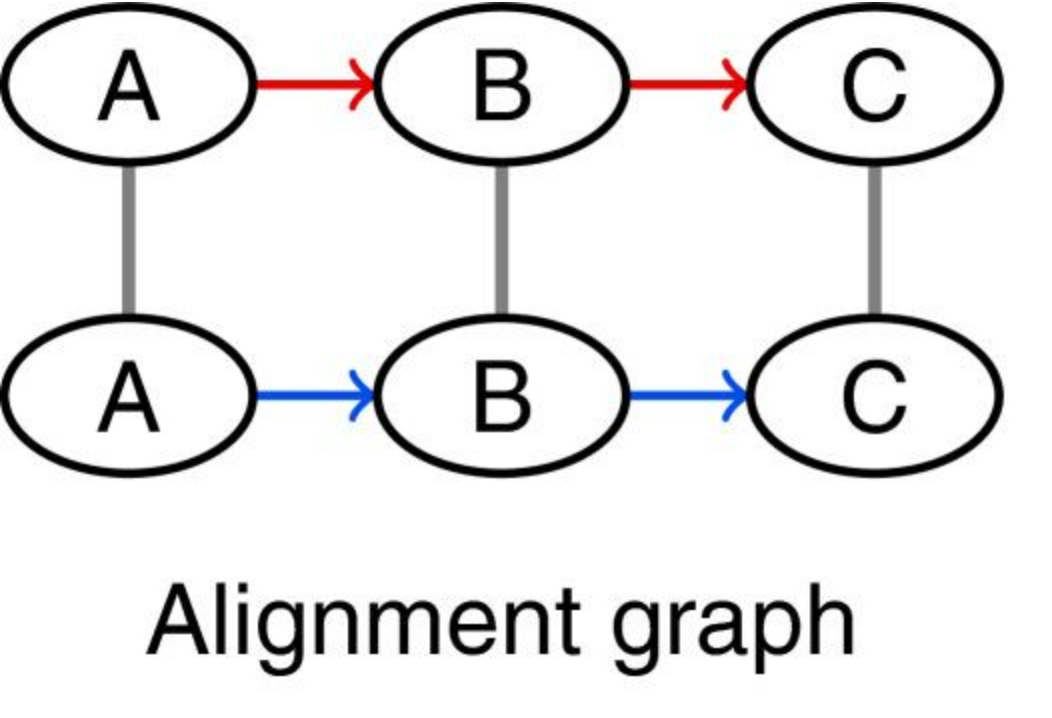
\includegraphics[scale=0.7,center]{alignmentgraph.png}
\end{figure}

{\footnotesize \url{https://bmcbioinformatics.biomedcentral.com/articles/10.1186/1471-2105-15-99}}

\end{columns}



\end{frame}

\begin{frame}
  \frametitle{Seqwish variation graph inducer}
  \begin{columns}[c] % The "c" option specifies centered vertical alignment while the "t" option is used for top vertical alignment

    \column{.45\textwidth} % Right column and width
    %Alignments of whole genomes are equivalently represented as a graph.
    Seqwish uses disk-backed algorithms to compute the full alignment graph and compact it into a variation graph.
    \\~\\
    Here, the variation graph induced by seqwish from the  minimap2 alignments of seven \emph{S. cerevisiae} genomes.
    (Note that alignments were filtered for length using \url{https://github.com/natir/fpa}.)
    \\~\\
    10.1038/ng.3847
    \column{.5\textwidth} % Left column and width

    \begin{figure}
      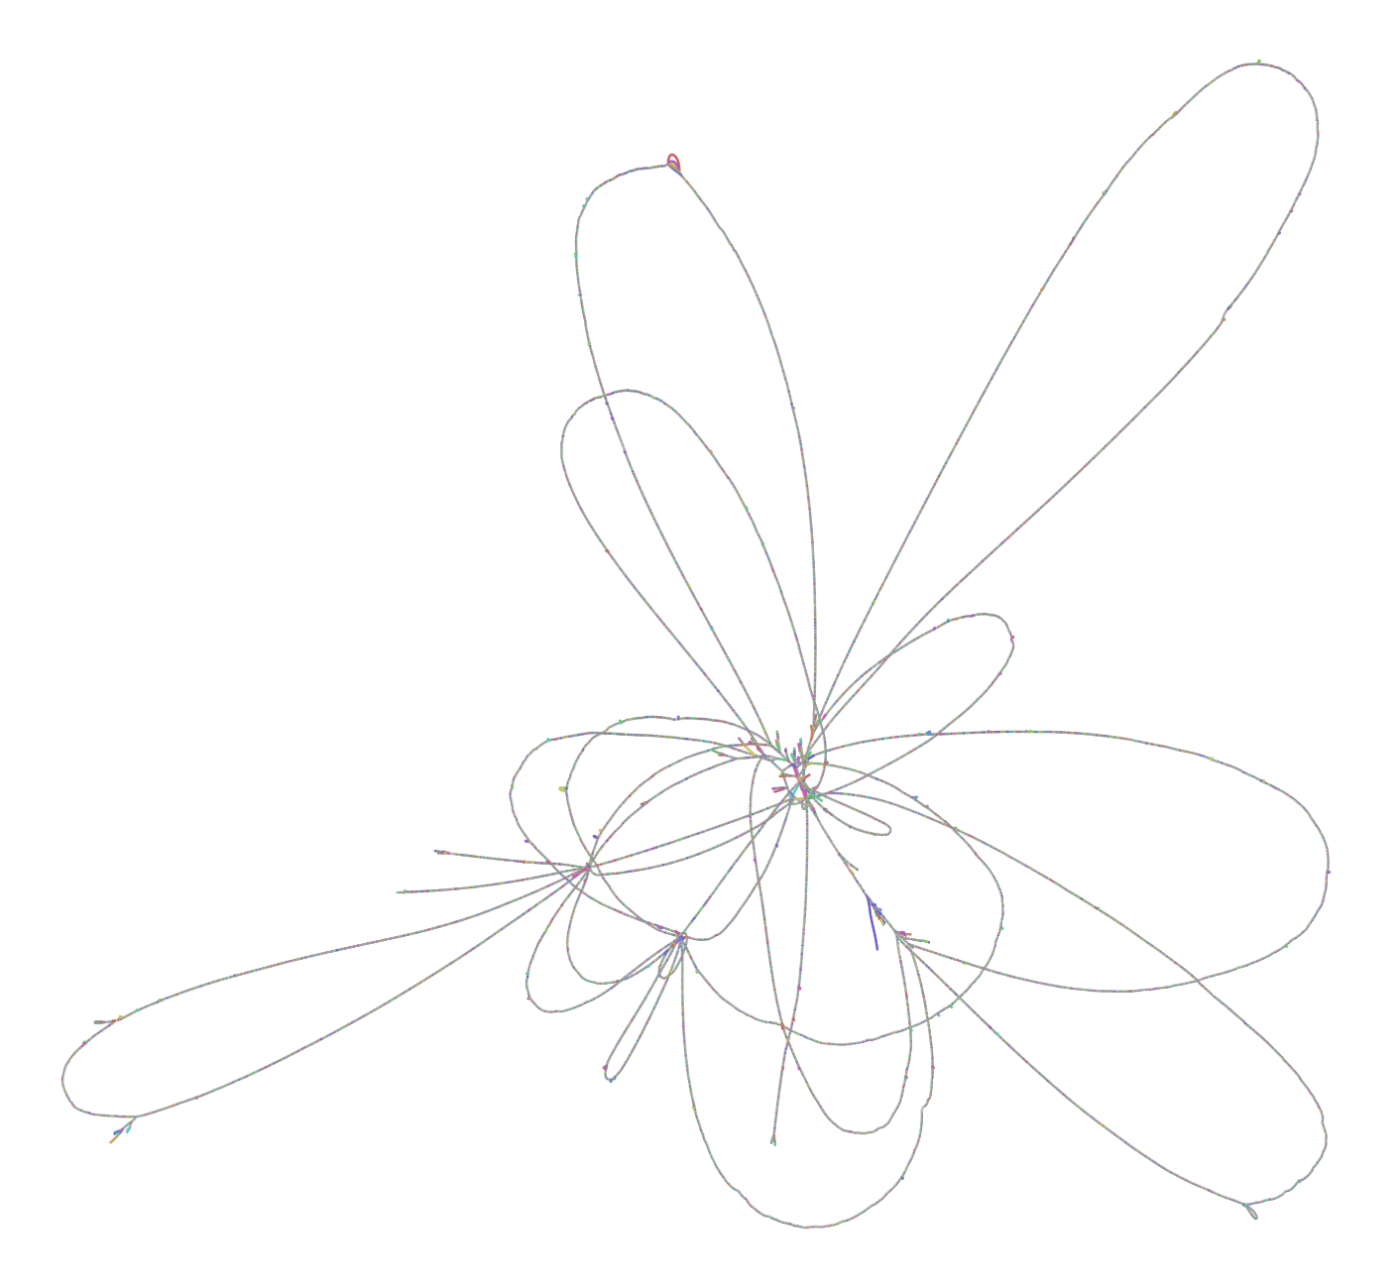
\includegraphics[scale=0.145,center]{seqwish_yeast.png}
    \end{figure}
  \end{columns}
\end{frame}

\section{Cichlid chr1 variation graph}
\begin{frame}
  \frametitle{Inducing the variation graph}
  Using chr1 from Acal, Mzeb, and Onil, align with minimap2, filter alignments by length (or not) and induce the variation graph with seqwish.
  \\~\\
  Approximately 10 minutes to build the alignmentset with minimap2 -c -x asm20.
  \\~\\
  Approximately 10 minutes to induce the graph with seqwish.
\end{frame}


\begin{frame}
  \frametitle{Cichlid chr1 unfiltered}
    \begin{figure}
      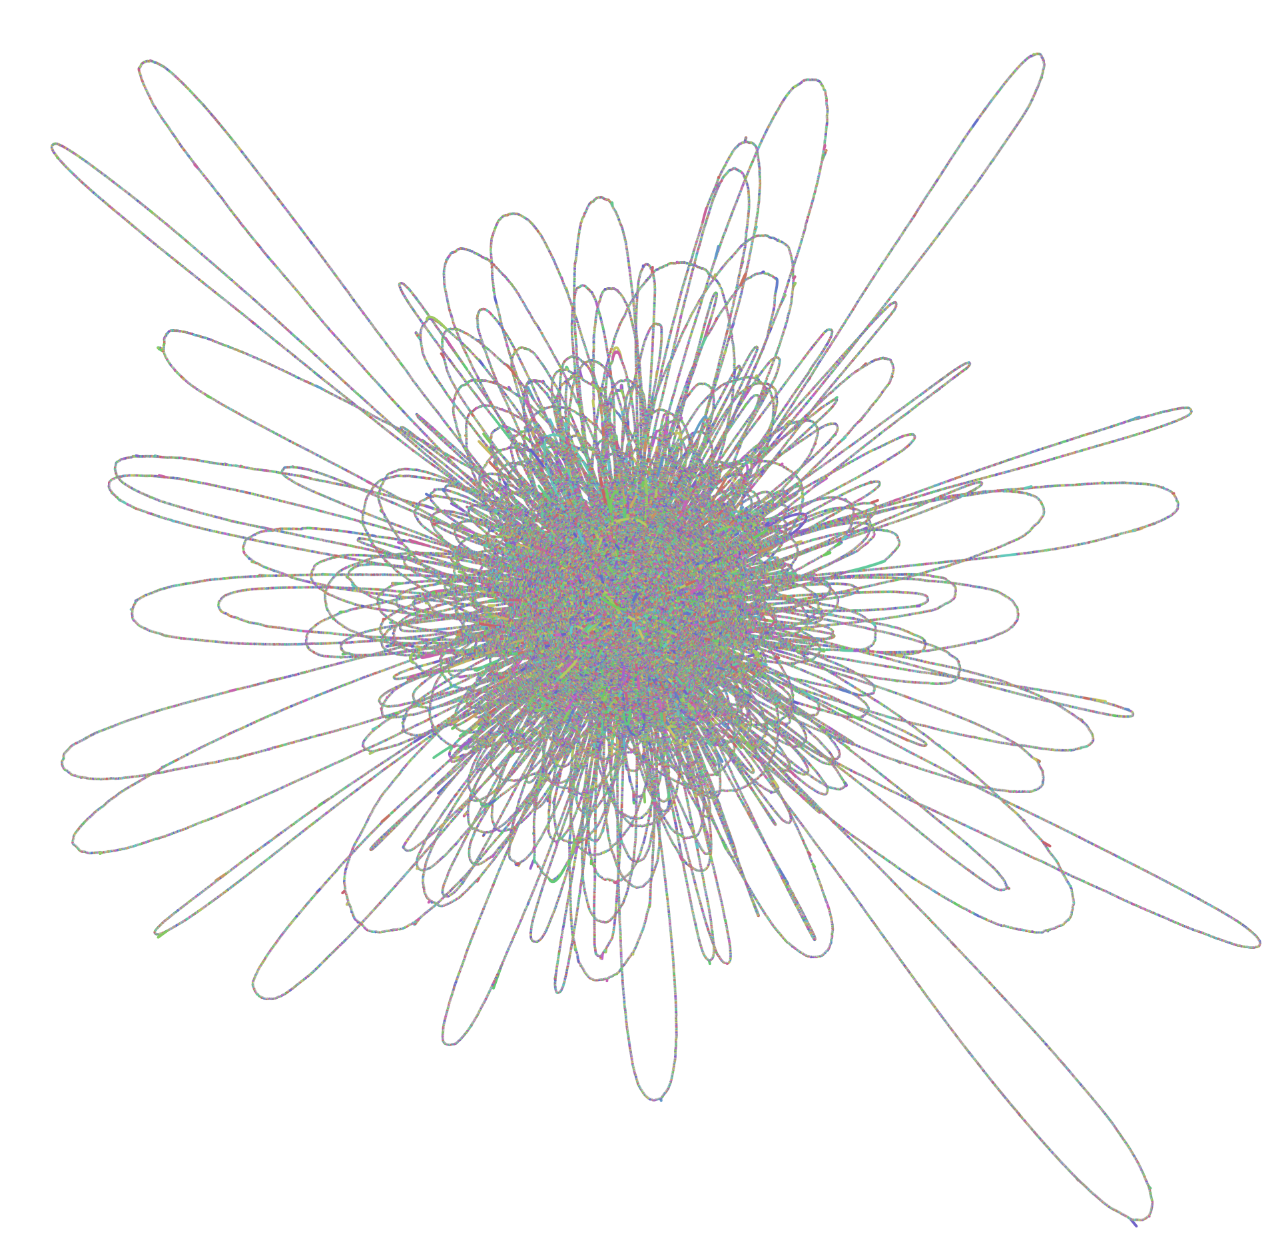
\includegraphics[scale=0.17,center]{seqwish-cichlid-chr1.png}
    \end{figure}
\end{frame}

\begin{frame}
  \frametitle{Cichlid chr1 filtered with fpa -l 2k}
    \begin{figure}
      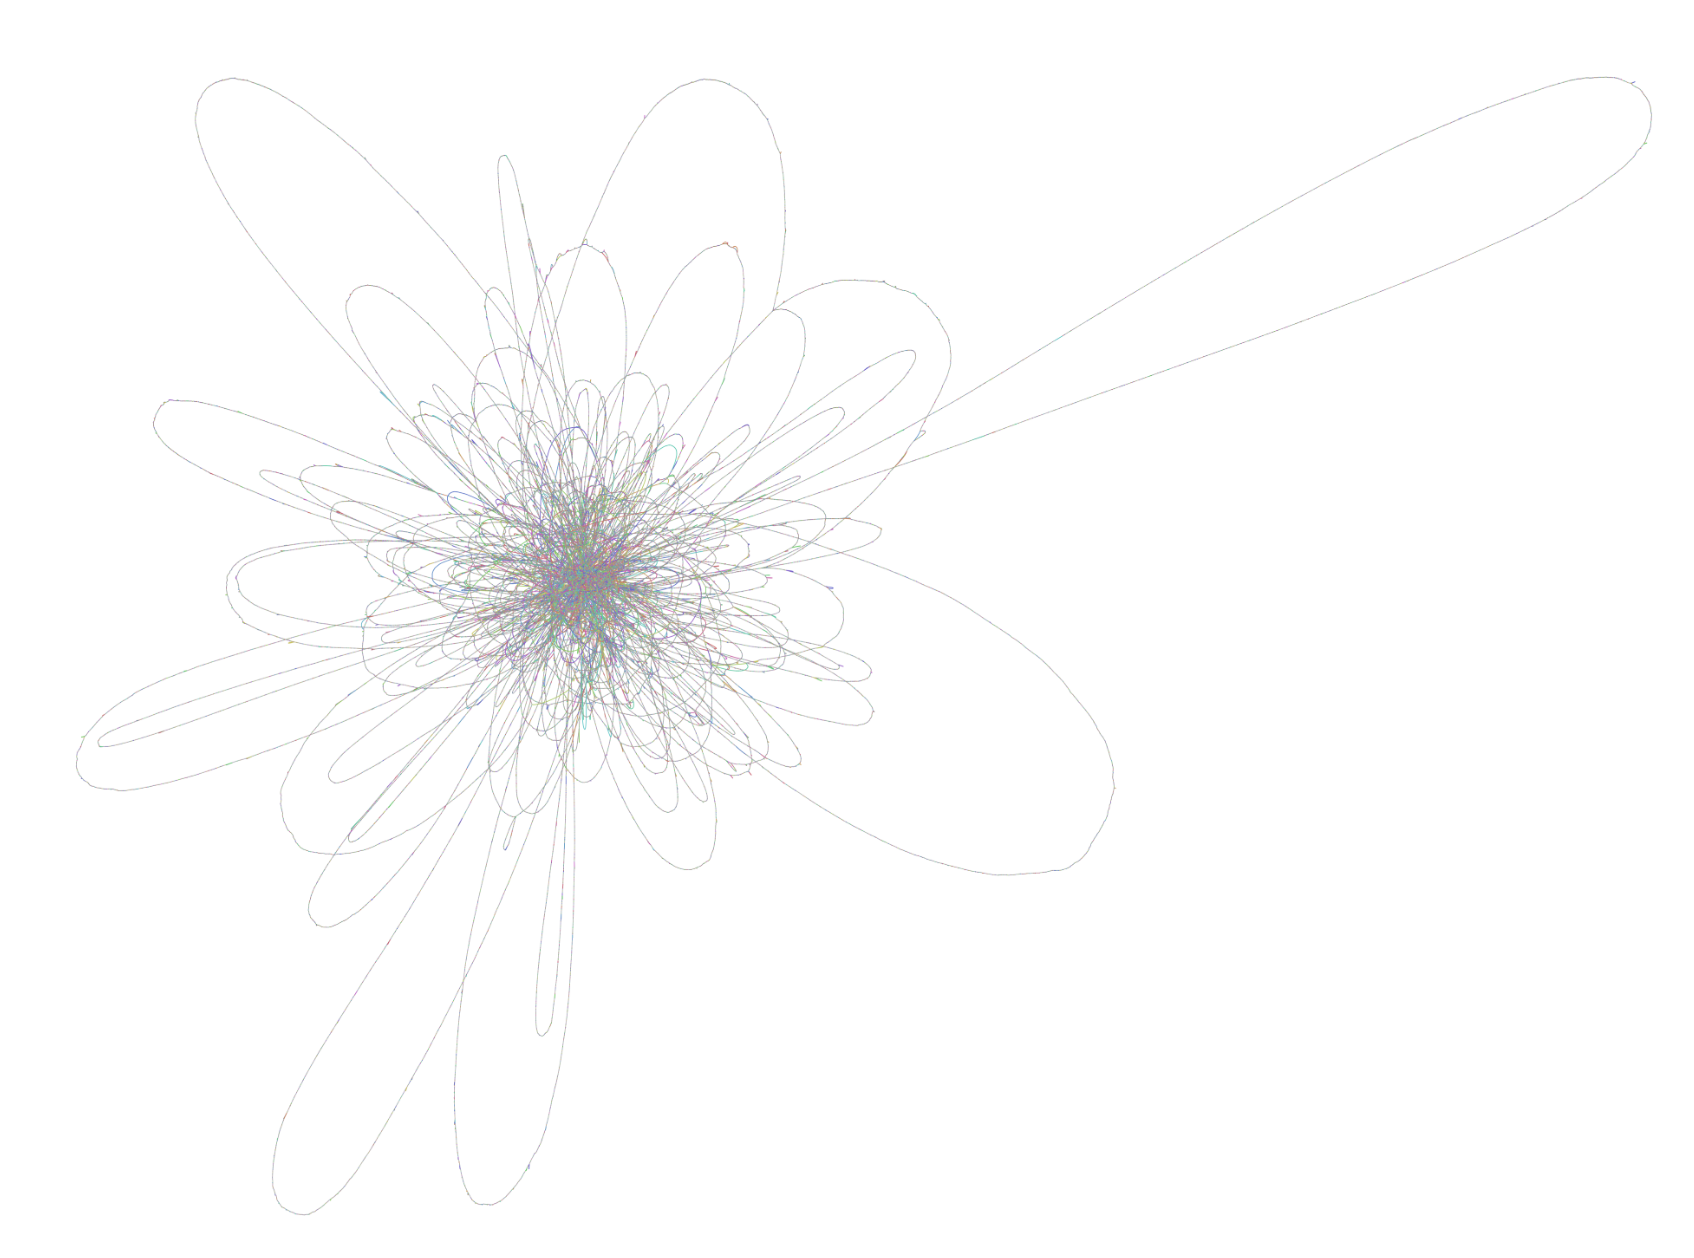
\includegraphics[scale=0.17,center]{seqwish-cichlid-chr1-fpal2k.png}
    \end{figure}
\end{frame}

\begin{frame}
  \frametitle{Cichlid chr1 filtered with fpa -l 10k}
    \begin{figure}
      
\includegraphics[scale=0.17,center]{seqwish-cichlid-chr1-fpal10k-1.png}
    \end{figure}
\end{frame}

\begin{frame}
  \frametitle{Cichlid chr1 filtered with fpa -l 10k (zoom)}
    \begin{figure}
      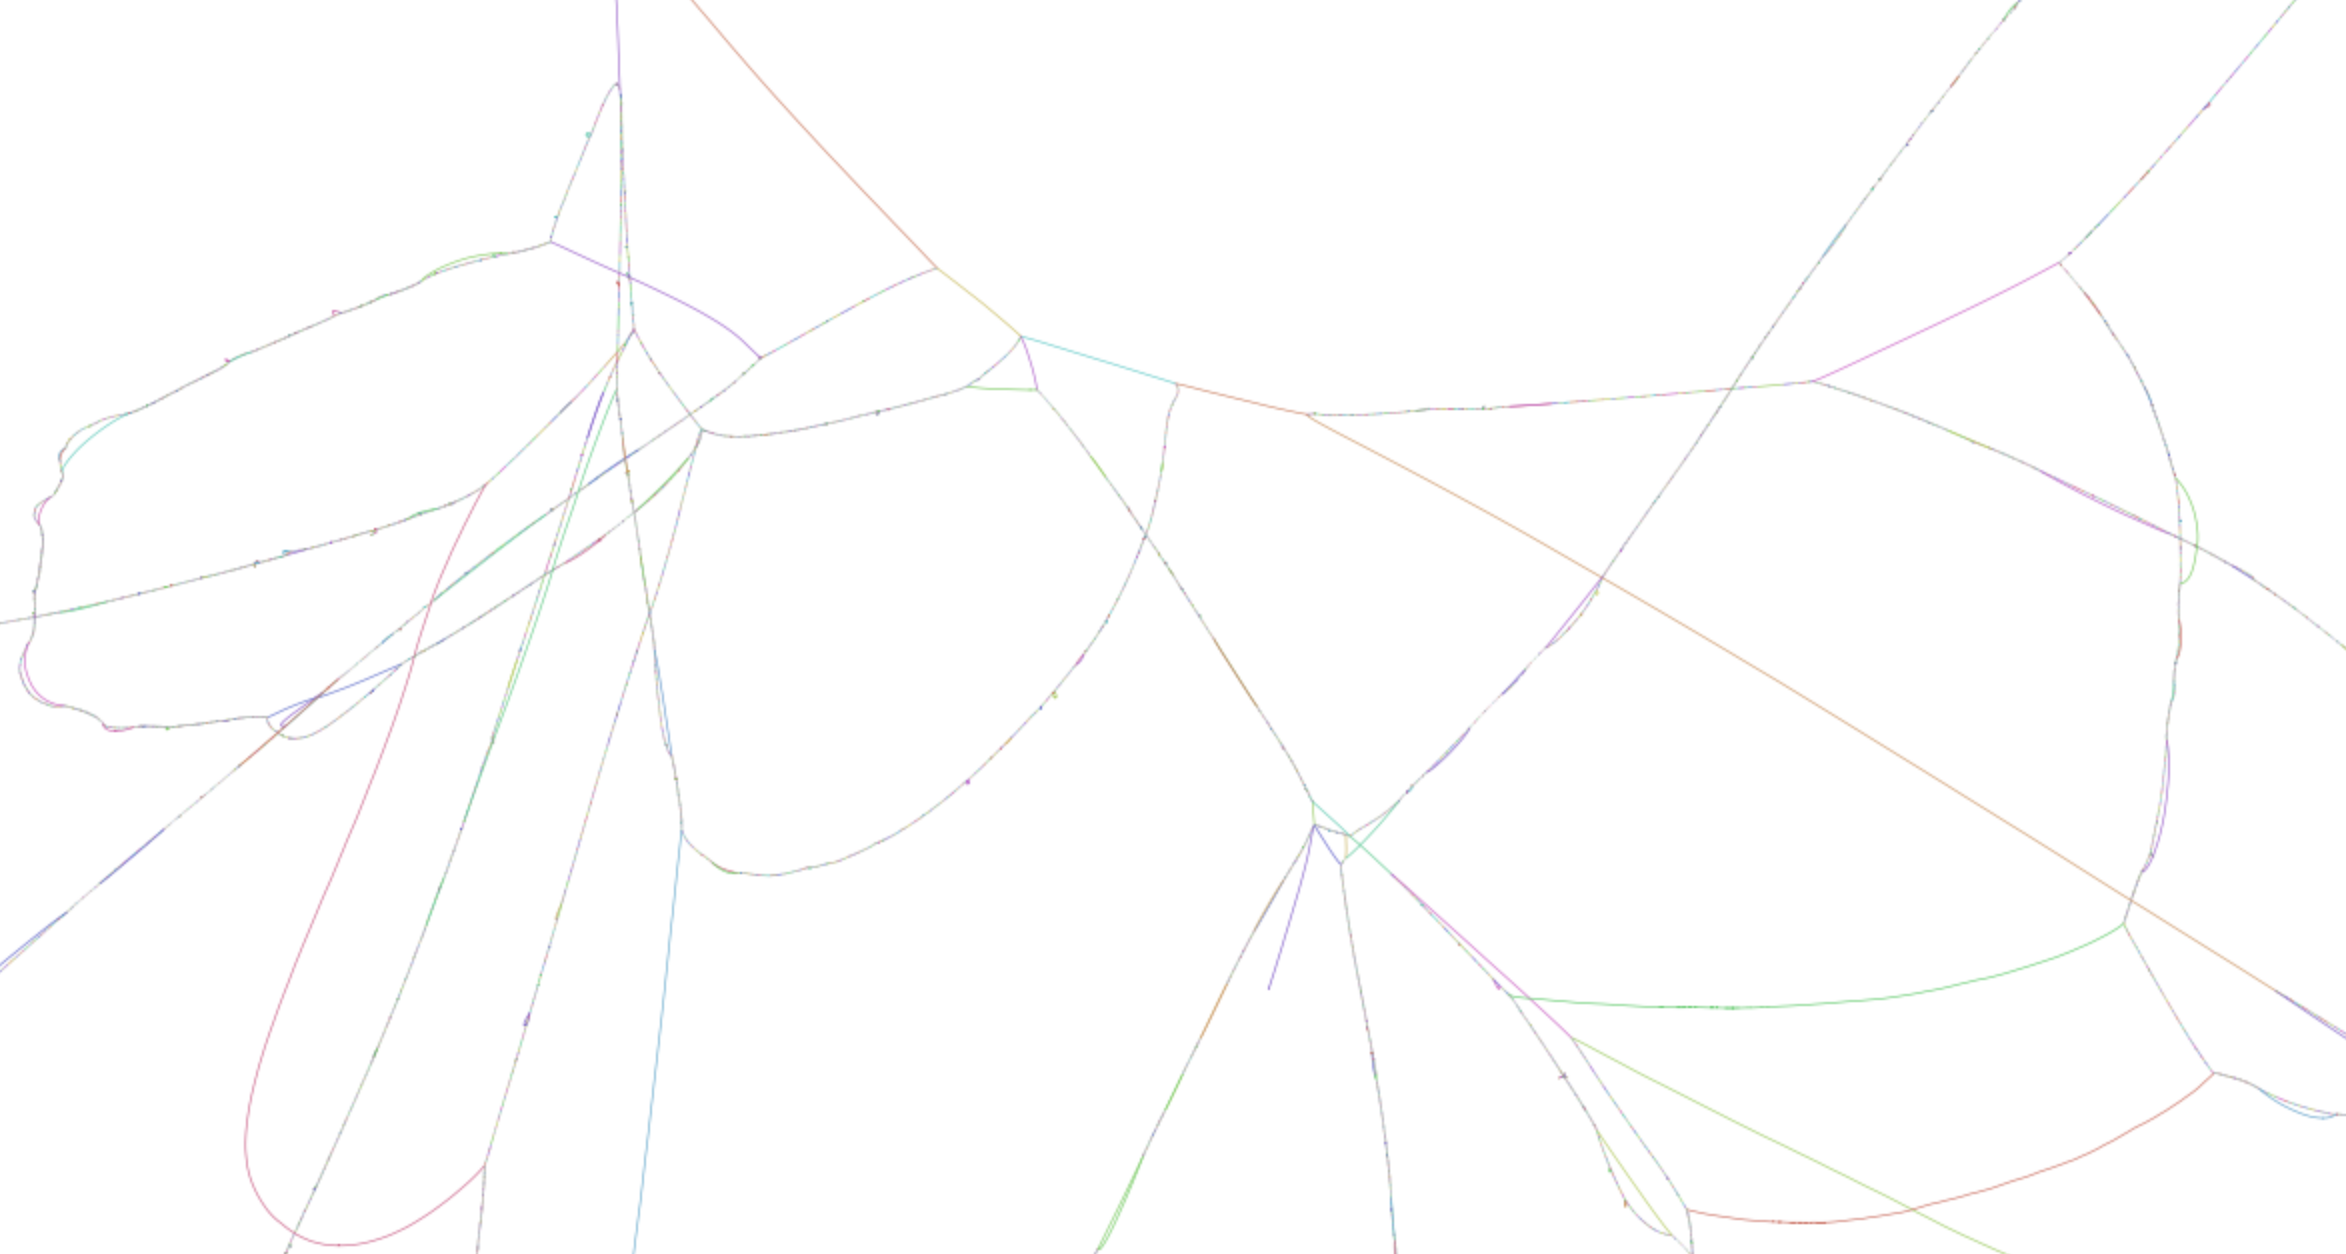
\includegraphics[scale=0.17,center]{seqwish-cichlid-chr1-fpal10k-2.png}
    \end{figure}
\end{frame}

\begin{frame}
  \frametitle{vg-dotplot of Acal vs. Mzeb}
    \begin{figure}
      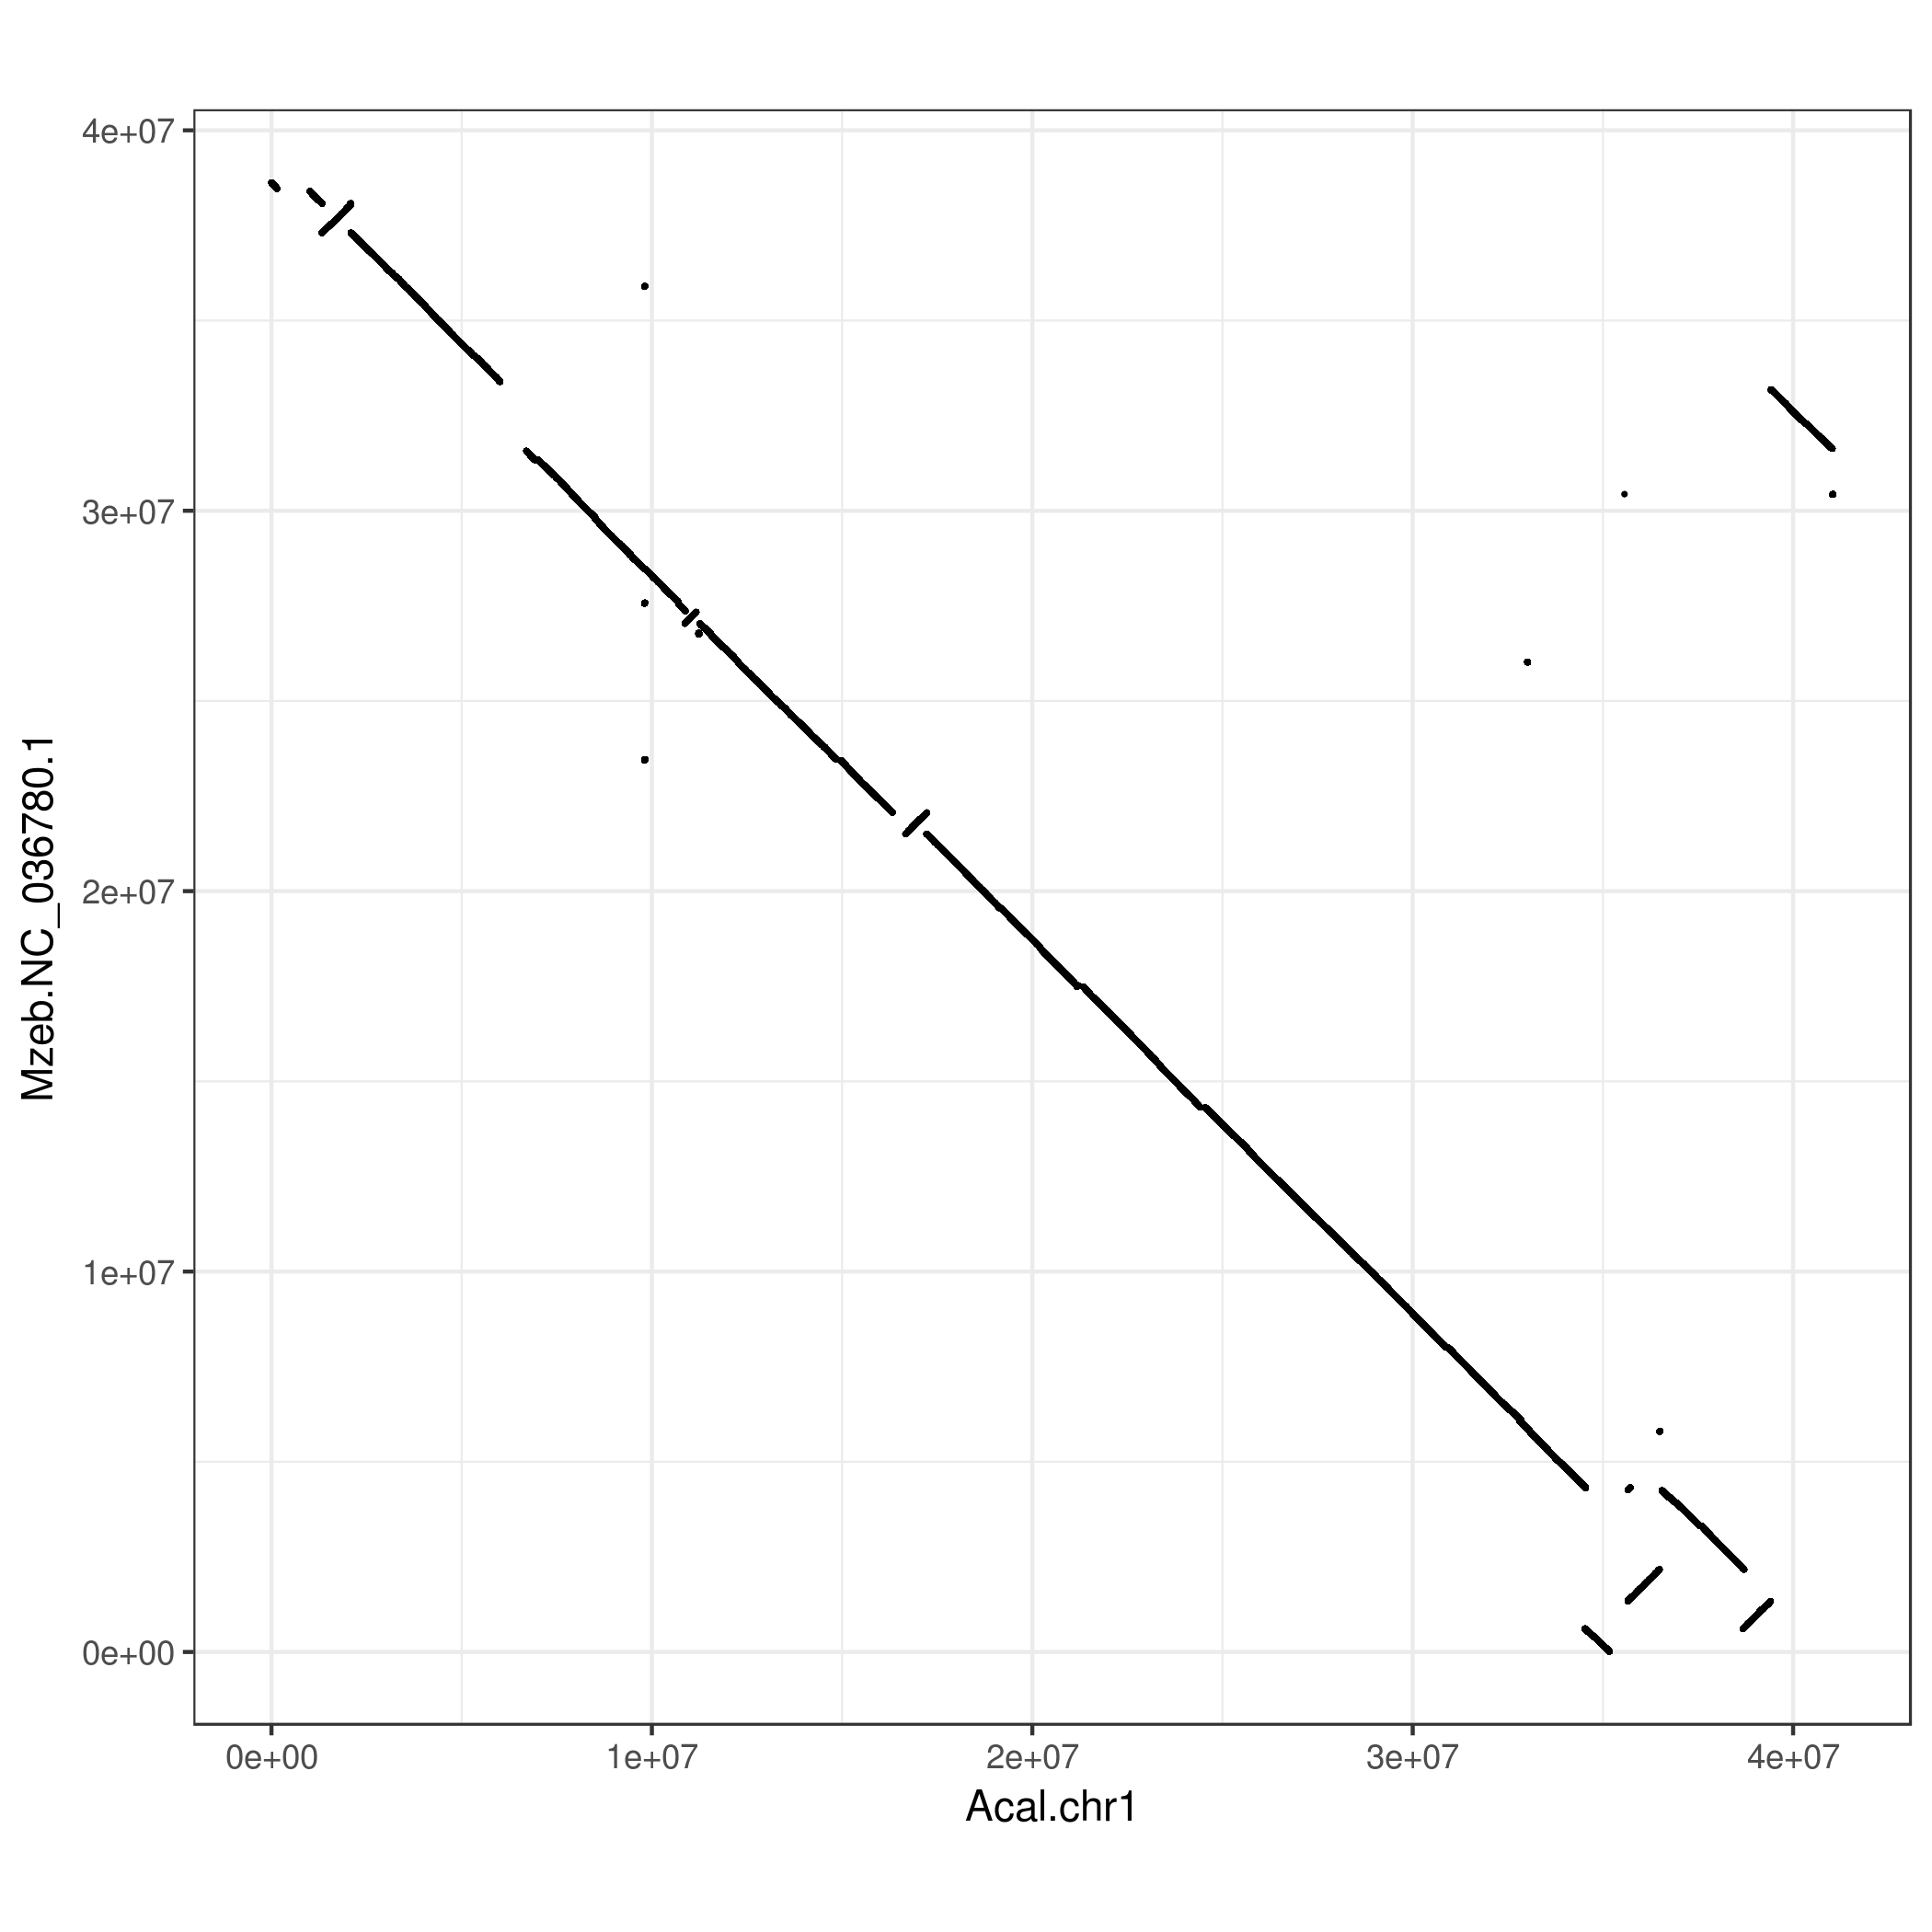
\includegraphics[scale=0.45,center]{Acal-Mzeb-dotplot.png}
    \end{figure}
\end{frame}

\begin{frame}
  \frametitle{vg-dotplot of Acal vs. Onil}
    \begin{figure}
      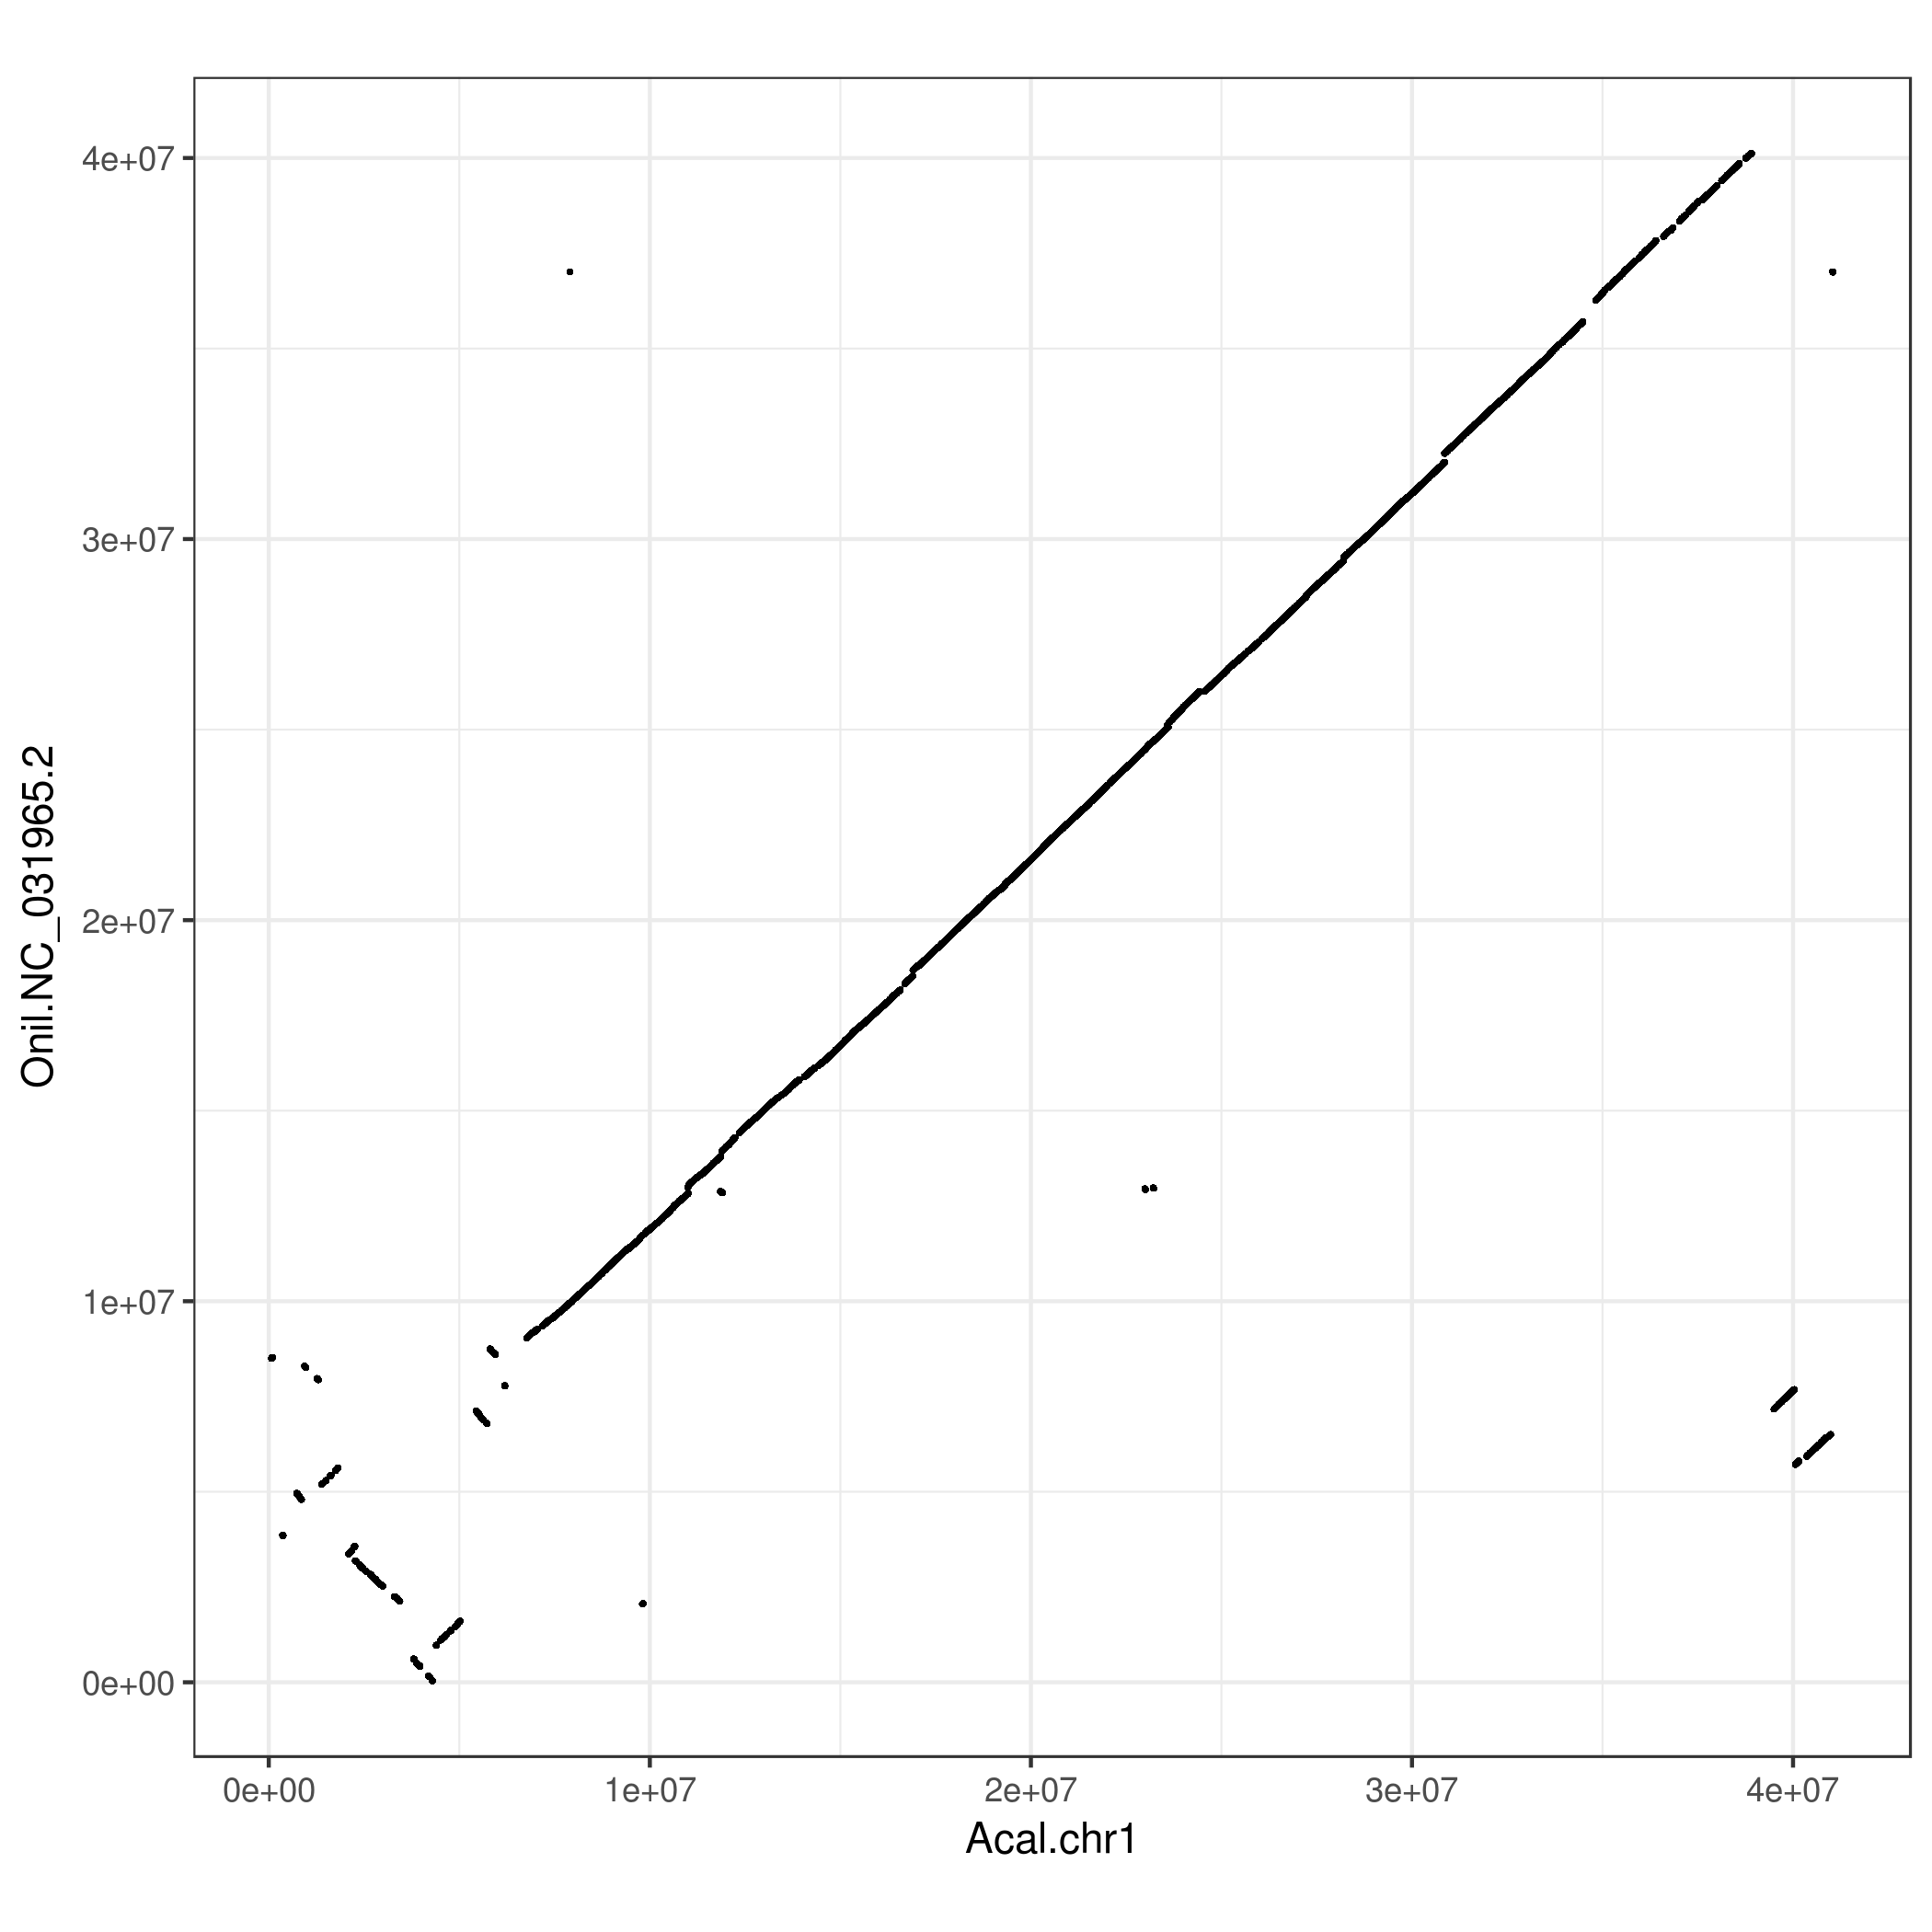
\includegraphics[scale=0.45,center]{Acal-Onil-dotplot.png}
    \end{figure}
\end{frame}

\begin{frame}
  \frametitle{vg-dotplot of Mzeb vs. Onil}
    \begin{figure}
      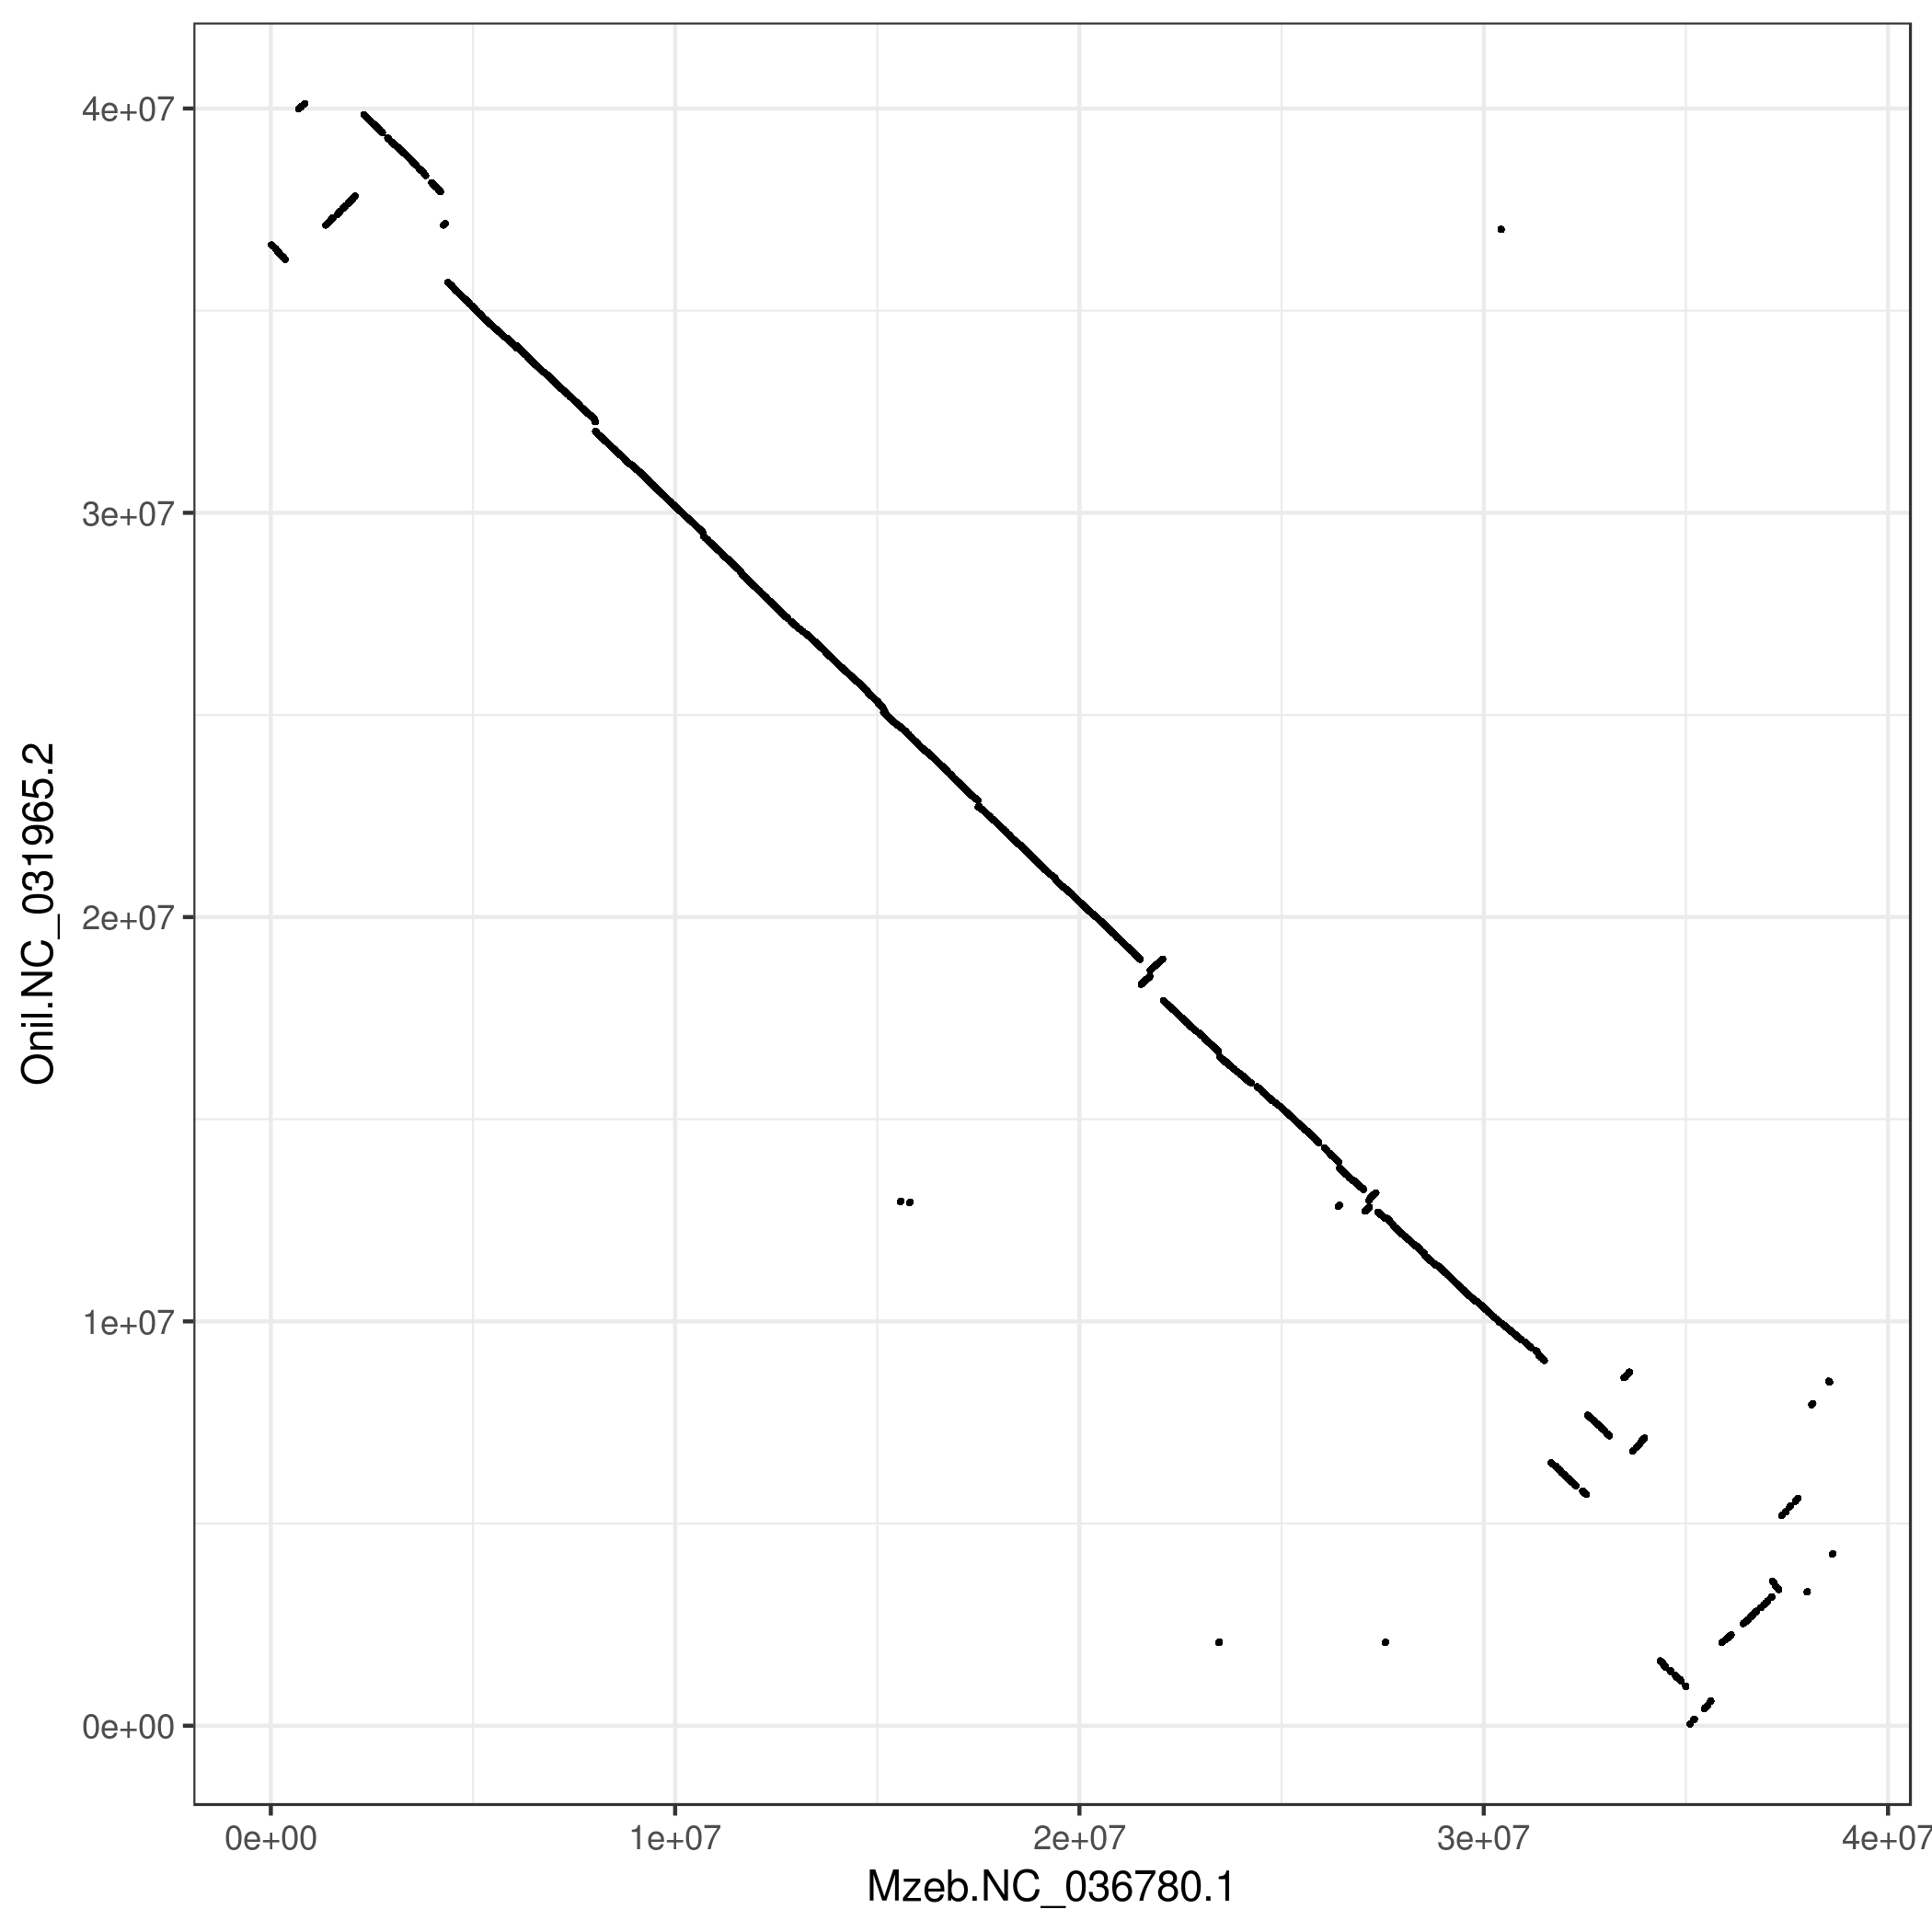
\includegraphics[scale=0.45,center]{Mzeb-Onil-dotplot.png}
    \end{figure}
\end{frame}

\section{BUSCO gene evaluation}
\begin{frame}
  \frametitle{Rationale}
  To determine the quality of these various approaches, we need some concept of the truth
  BUSCO single-copy orthologs are as good as we've got.
  \\~\\
  Here, the idea is to find the high-confidence orthologs in these chr1 assemblies and evaluate if they are:
  \begin{enumerate}
  \item \emph{Single-copy?} Are the BUSCO genes in the graph in regions of the graph where each input genome is contributing a single copy (there are no induced CNVs).
  \item \emph{Complete alignment?} Are the alignments of these genes to each other preserved in the graph? (they're orthologous)
  \end{enumerate}
  %\\~\\
  I'll be using busco\_actinopterygii\_odb9.
  I apply tblastn to align the ancestral proteins from this set to each chromosome, then filter for e-values below 1e-100.
\end{frame}

\begin{frame}
  \frametitle{Copy state in graph}
  Considering each alignment region, how many unique paths overlap it in the graph? How many total path steps?
\end{frame}

\begin{frame}
  \frametitle{Copy state in graph, unfiltered}
  \begin{columns}[c] % The "c" option specifies centered vertical alignment while the "t" option is used for top vertical alignment
    \column{.35\textwidth} % Right column and width
    For Acal, 0.976 are in 3-way uniques.
    For Mzeb, 0.762.
    For Onil, 0.764.
    \column{.45\textwidth} % Right column and width
    \begin{figure}
      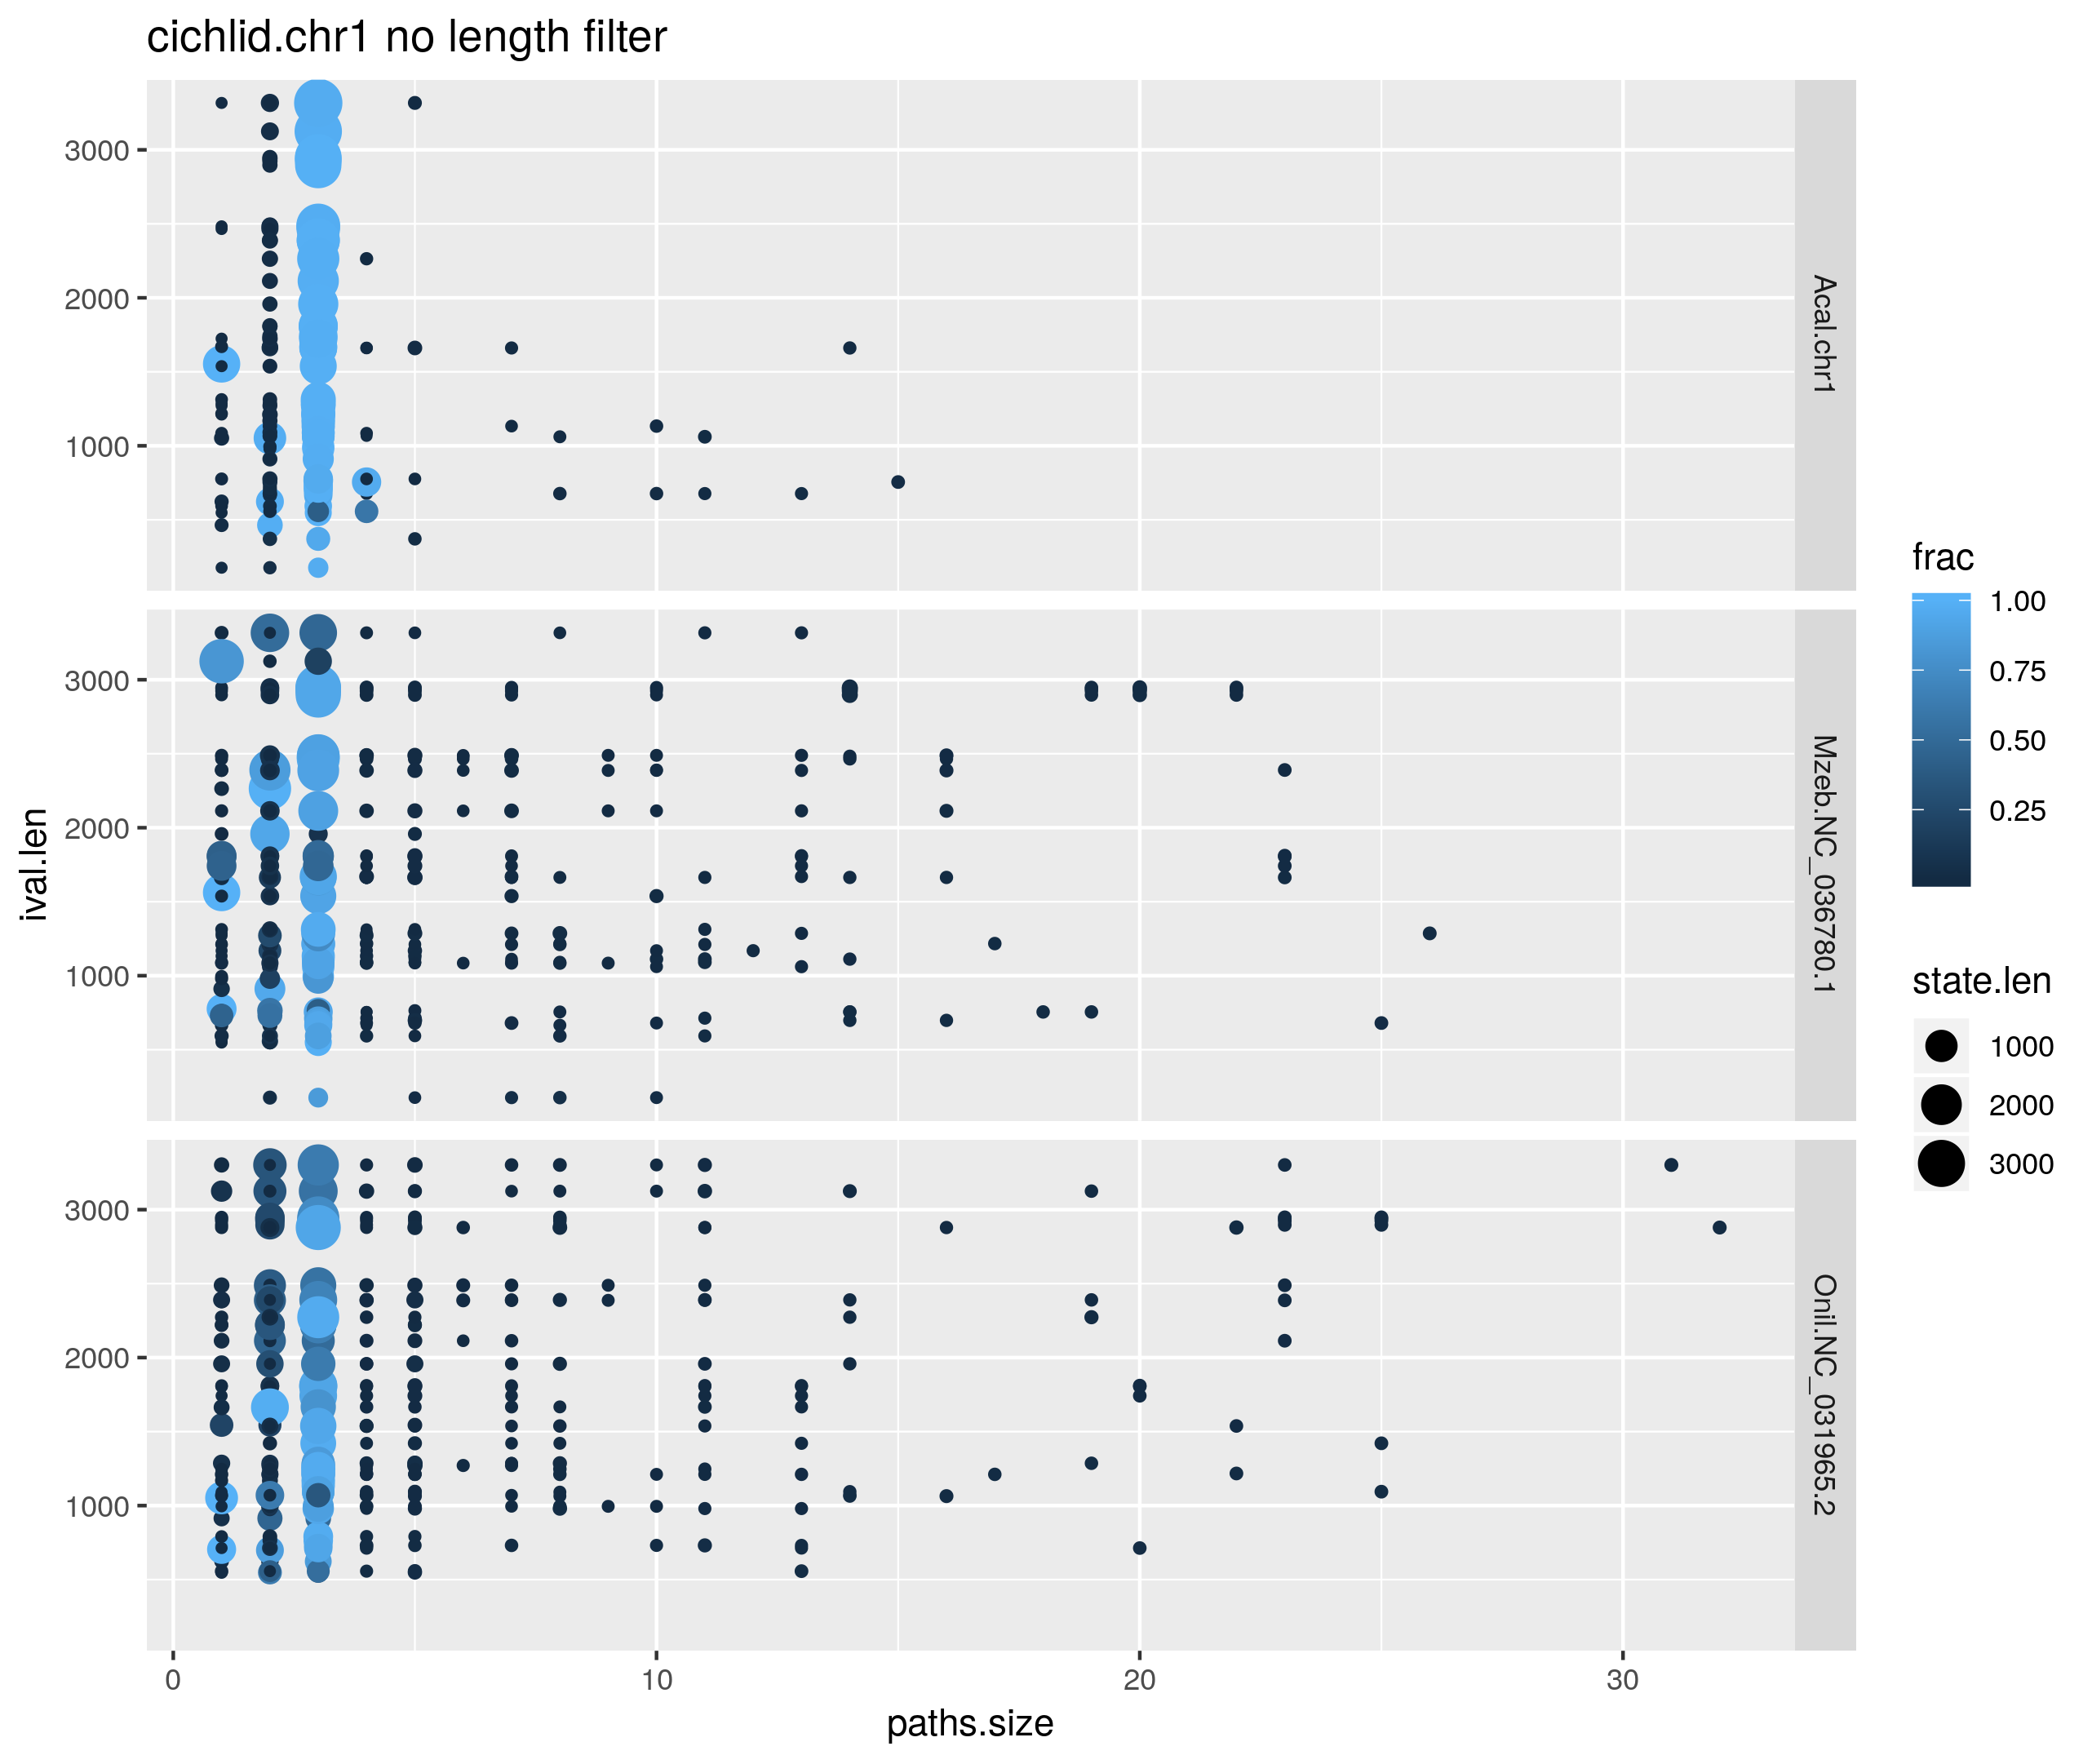
\includegraphics[scale=0.42,center]{cichlid_chr1_busco_multicov_len_vs_path_size.png}
    \end{figure}
  \end{columns}
\end{frame}

\begin{frame}
  \frametitle{Copy state in graph, filtered less than 2kb}
  \begin{columns}[c] % The "c" option specifies centered vertical alignment while the "t" option is used for top vertical alignment
    \column{.35\textwidth} % Right column and width
    For Acal, 0.976 are in 3-way uniques.
    For Mzeb, 0.841.
    For Onil, 0.750.
    \column{.45\textwidth} % Right column and width
    \begin{figure}
      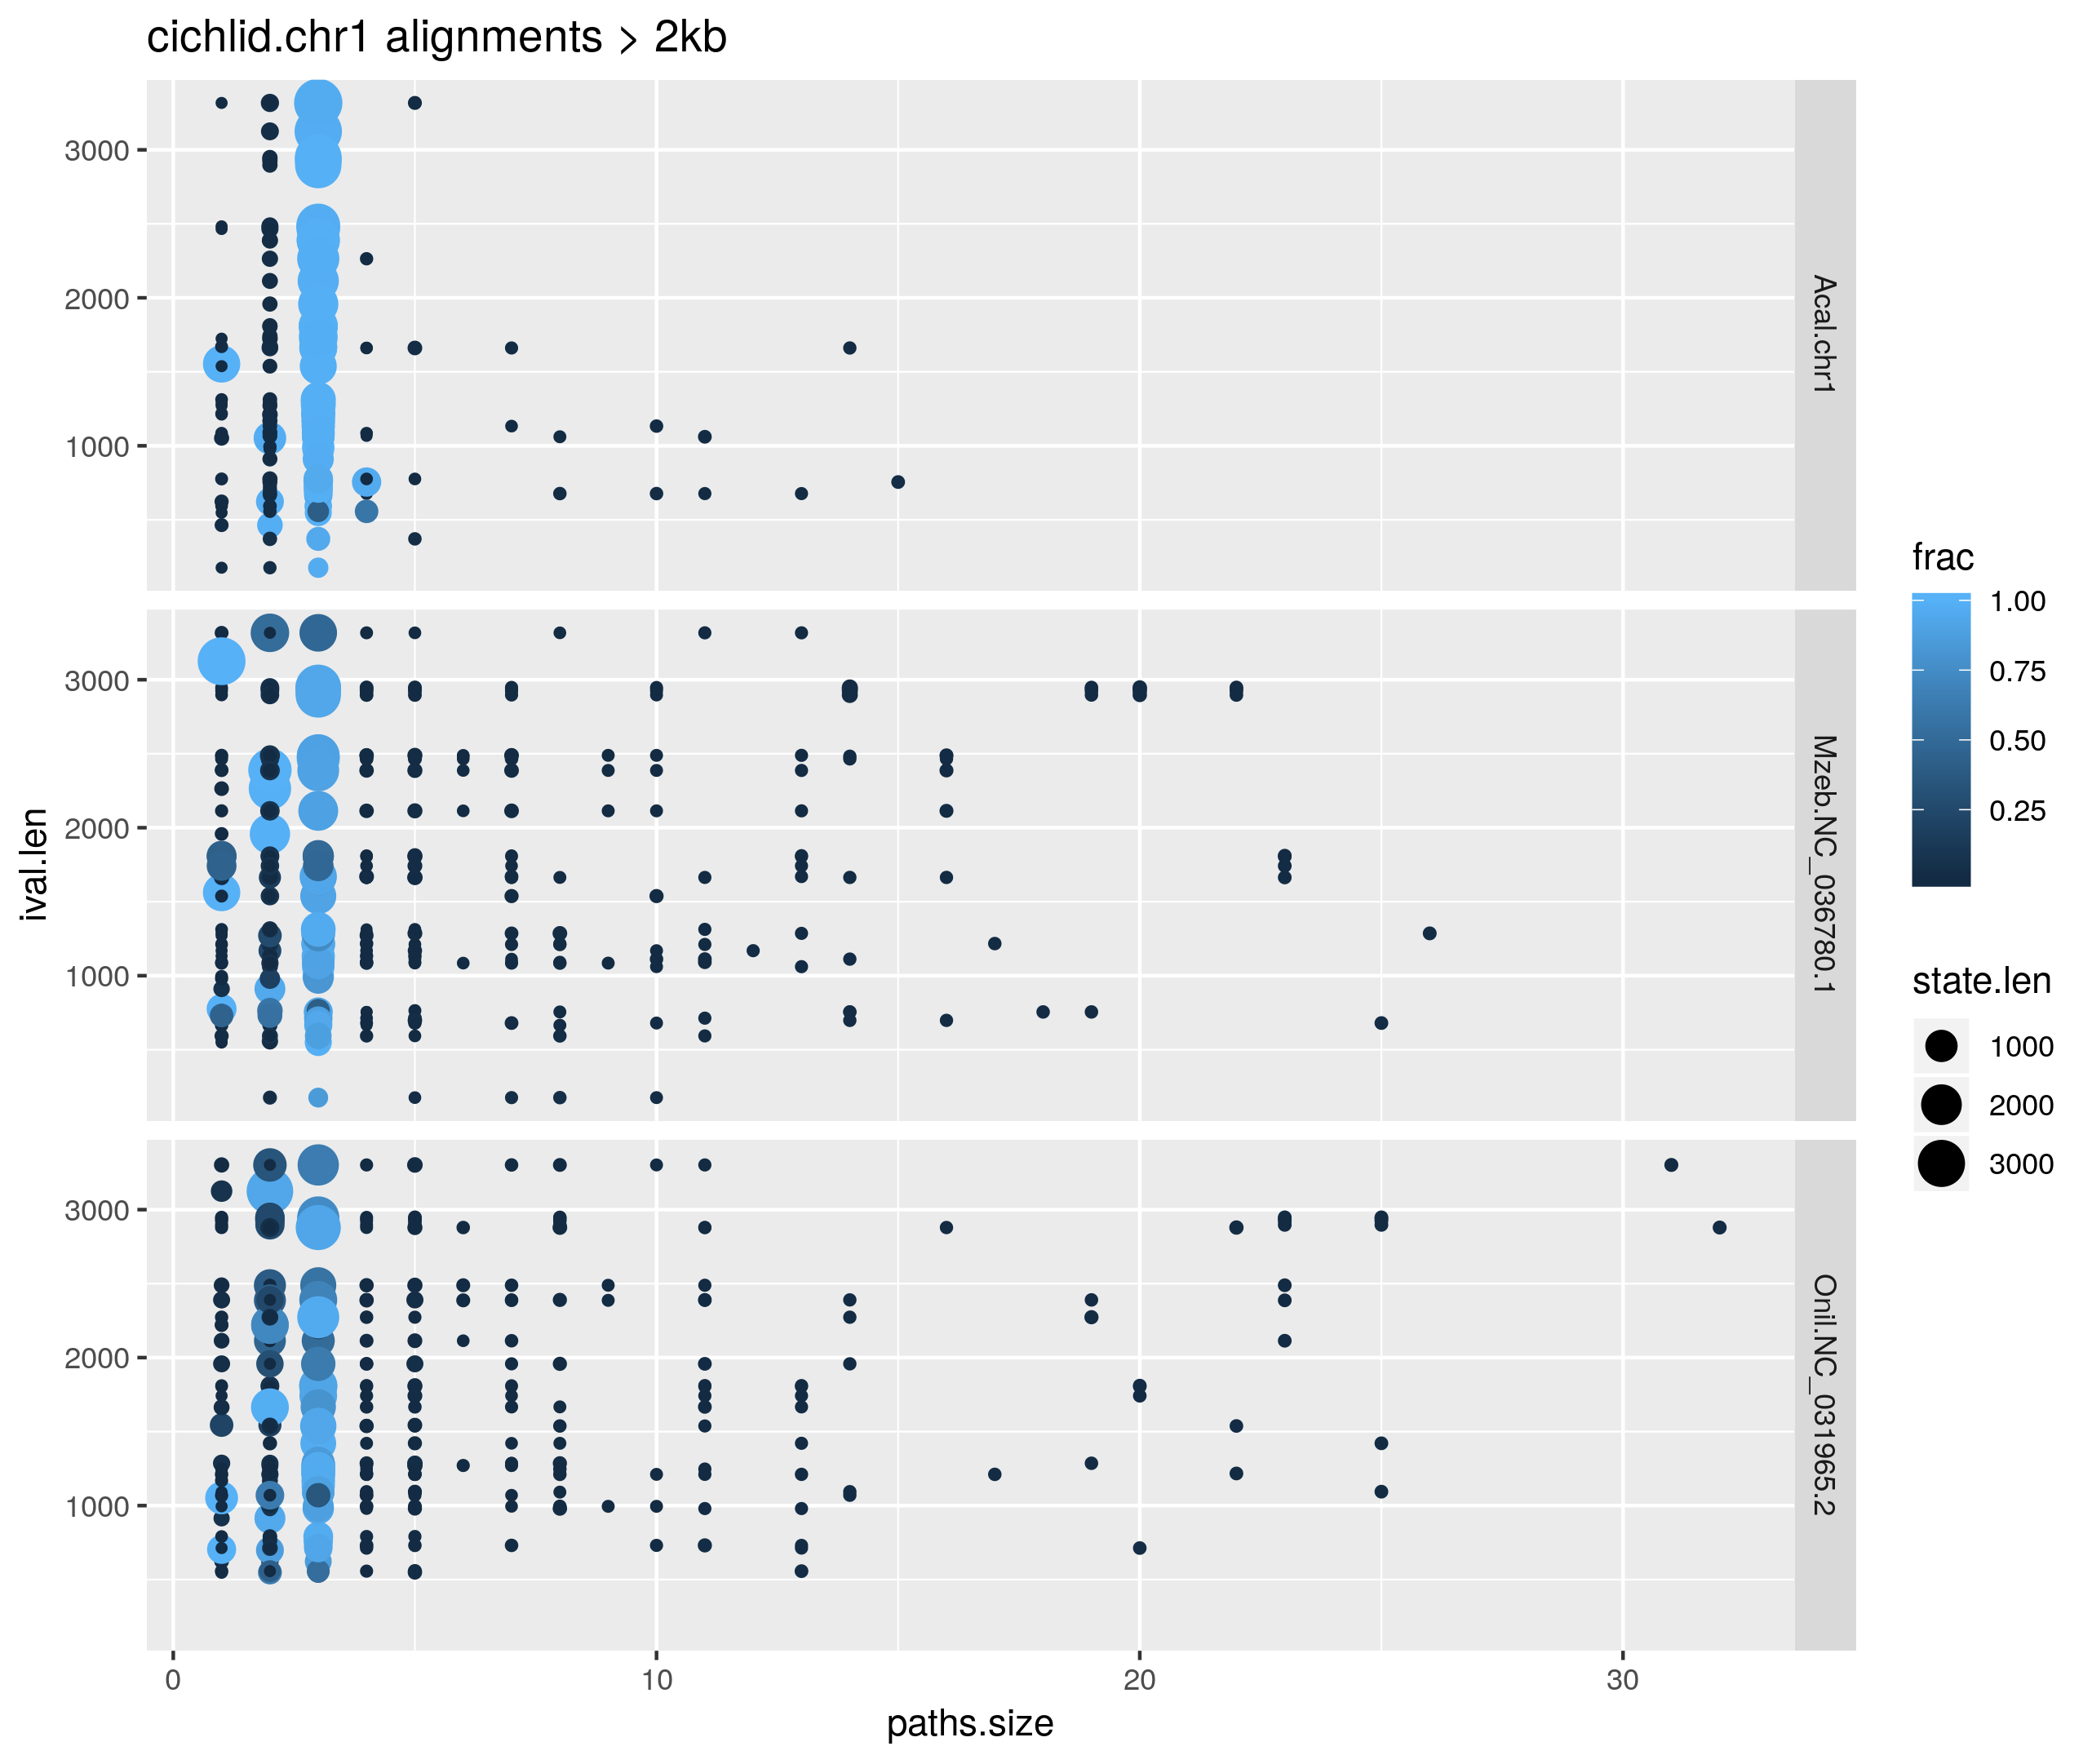
\includegraphics[scale=0.42,center]{cichlid_chr1_fpal2k_busco_multicov_len_vs_path_size.png}
    \end{figure}
    \end{columns}
\end{frame}

\begin{frame}
  \frametitle{Copy state in graph, filtered less than 10kb}
  \begin{columns}[c] % The "c" option specifies centered vertical alignment while the "t" option is used for top vertical alignment
    \column{.35\textwidth} % Right column and width
    For Acal, 0.981 are in 3-way uniques.
    For Mzeb, 0.847.
    For Onil, 0.798.
    \column{.45\textwidth} % Right column and width
    \begin{figure}
      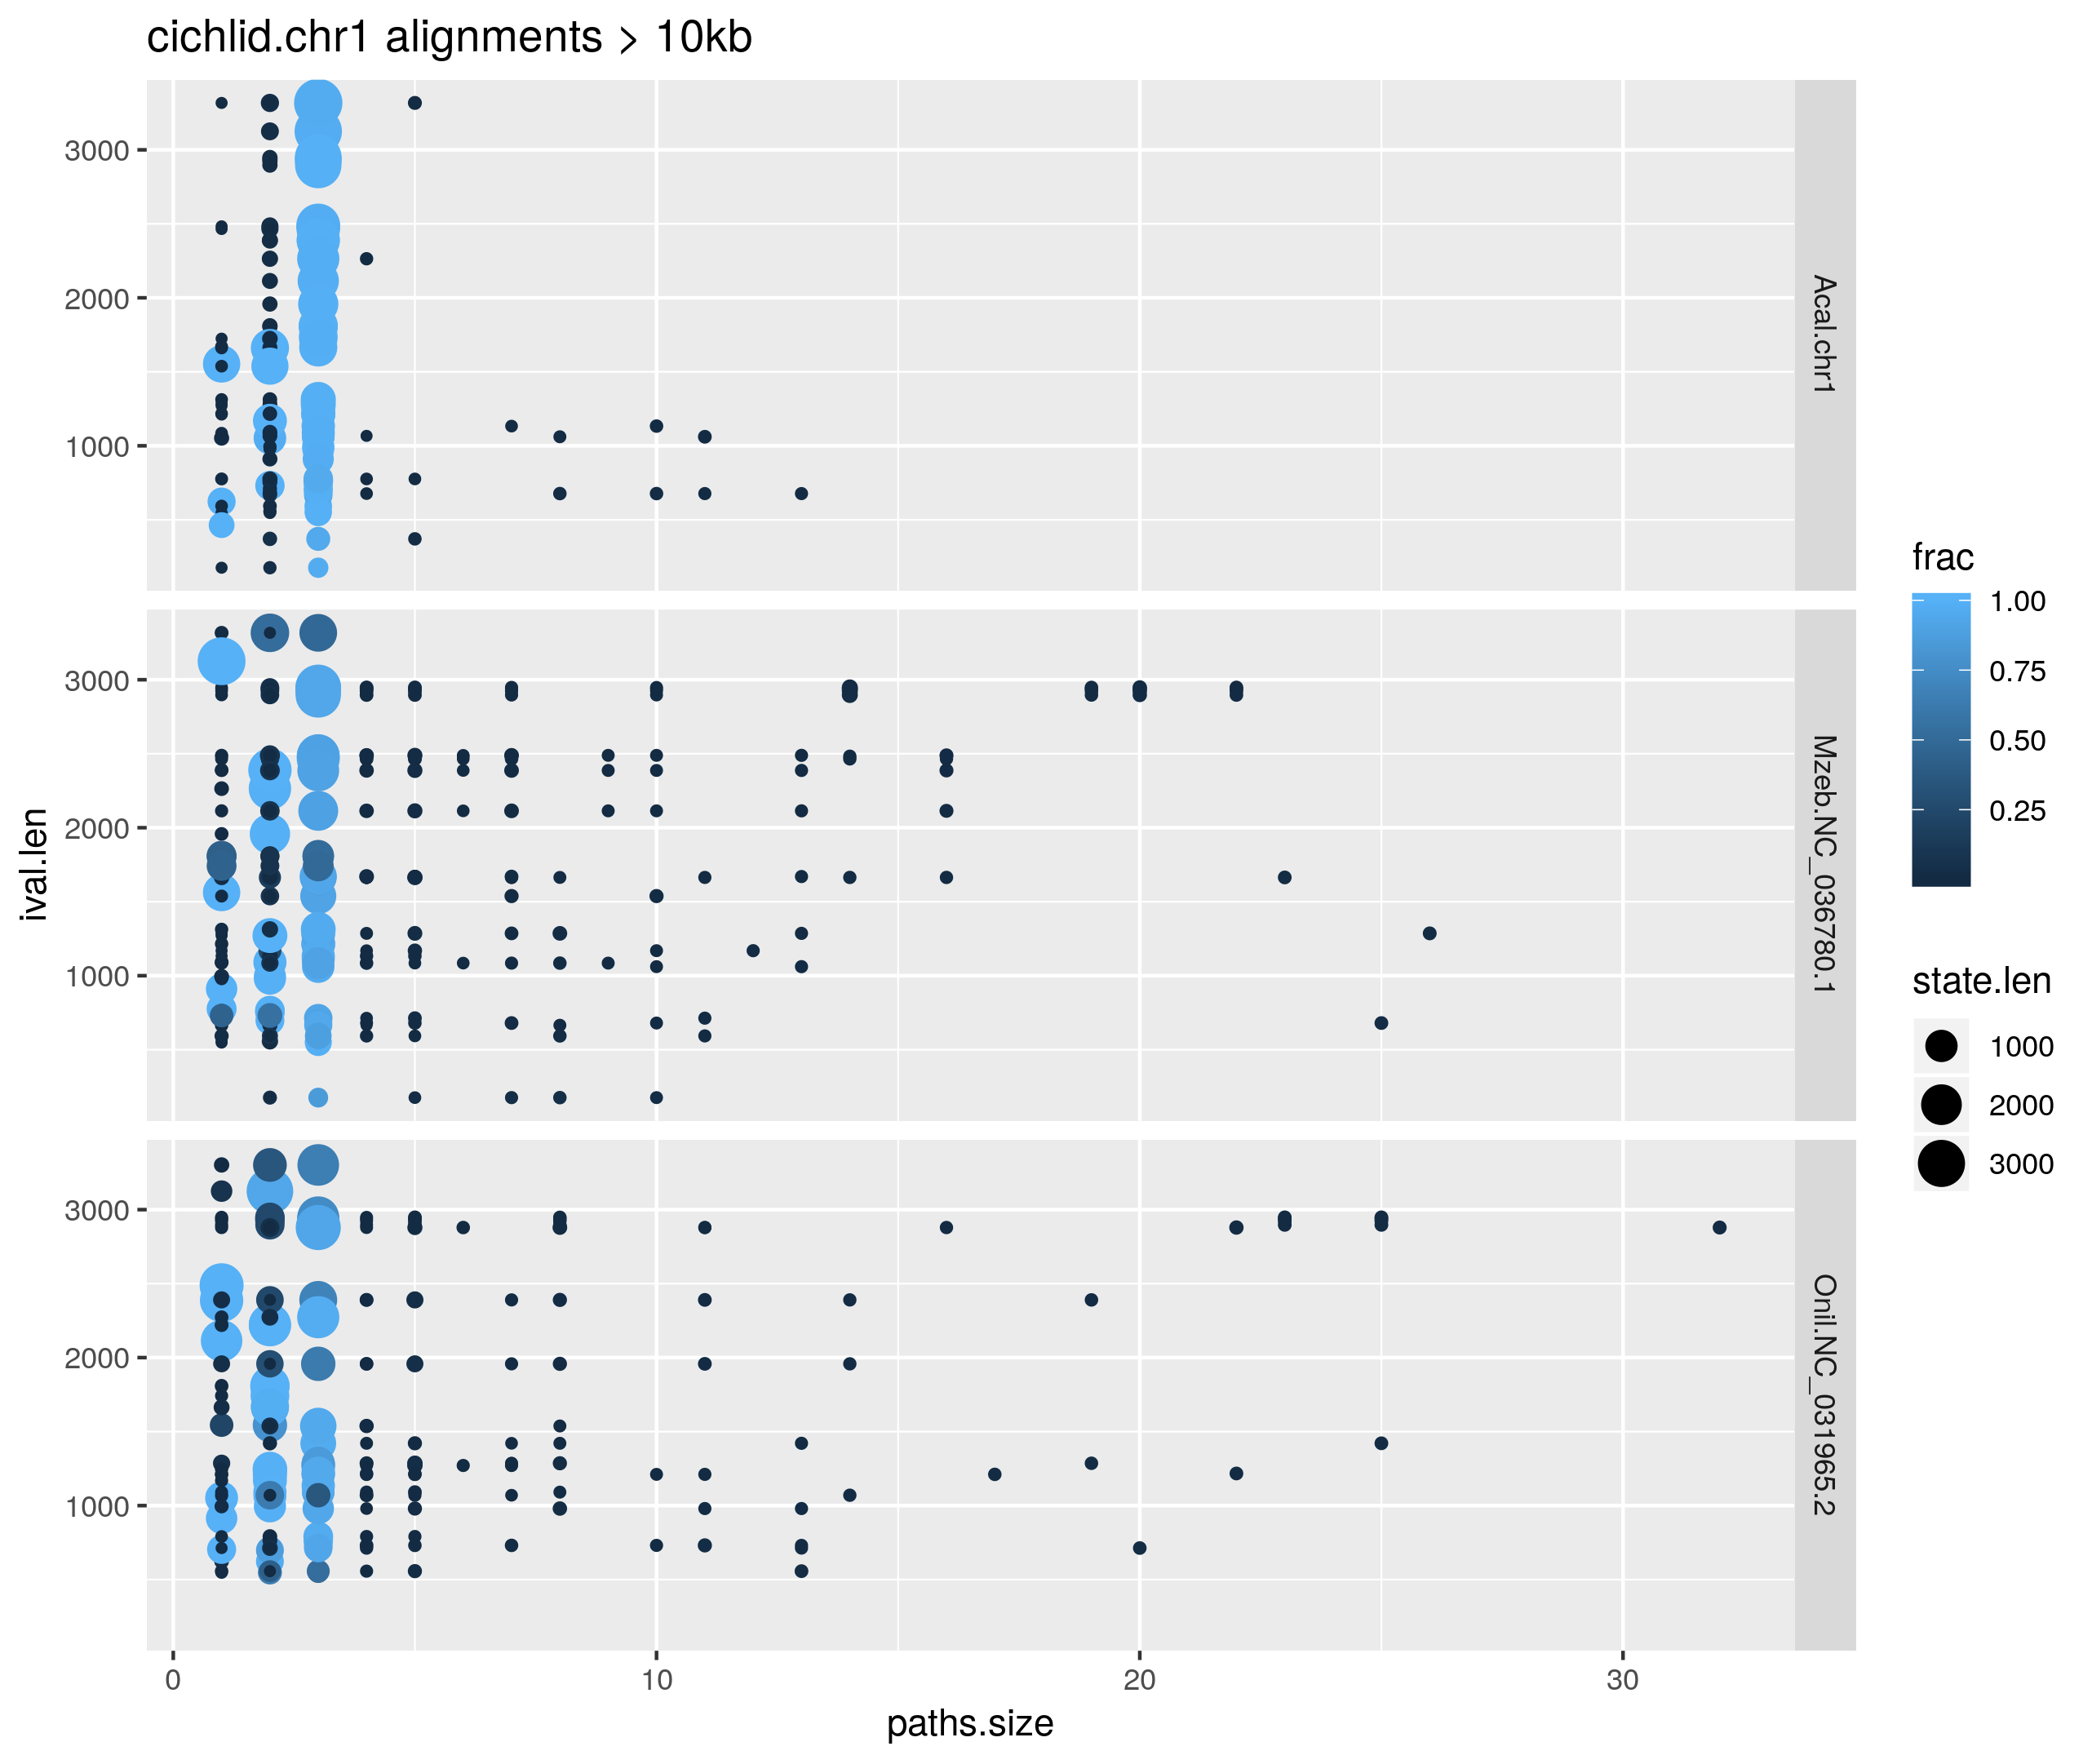
\includegraphics[scale=0.42,center]{cichlid_chr1_fpal10k_busco_multicov_len_vs_path_size.png}
    \end{figure}
  \end{columns}
\end{frame}

\begin{frame}
  \frametitle{BUSCO gene alignments from fpal10k graph, Acal vs Onil}
  \begin{figure}
    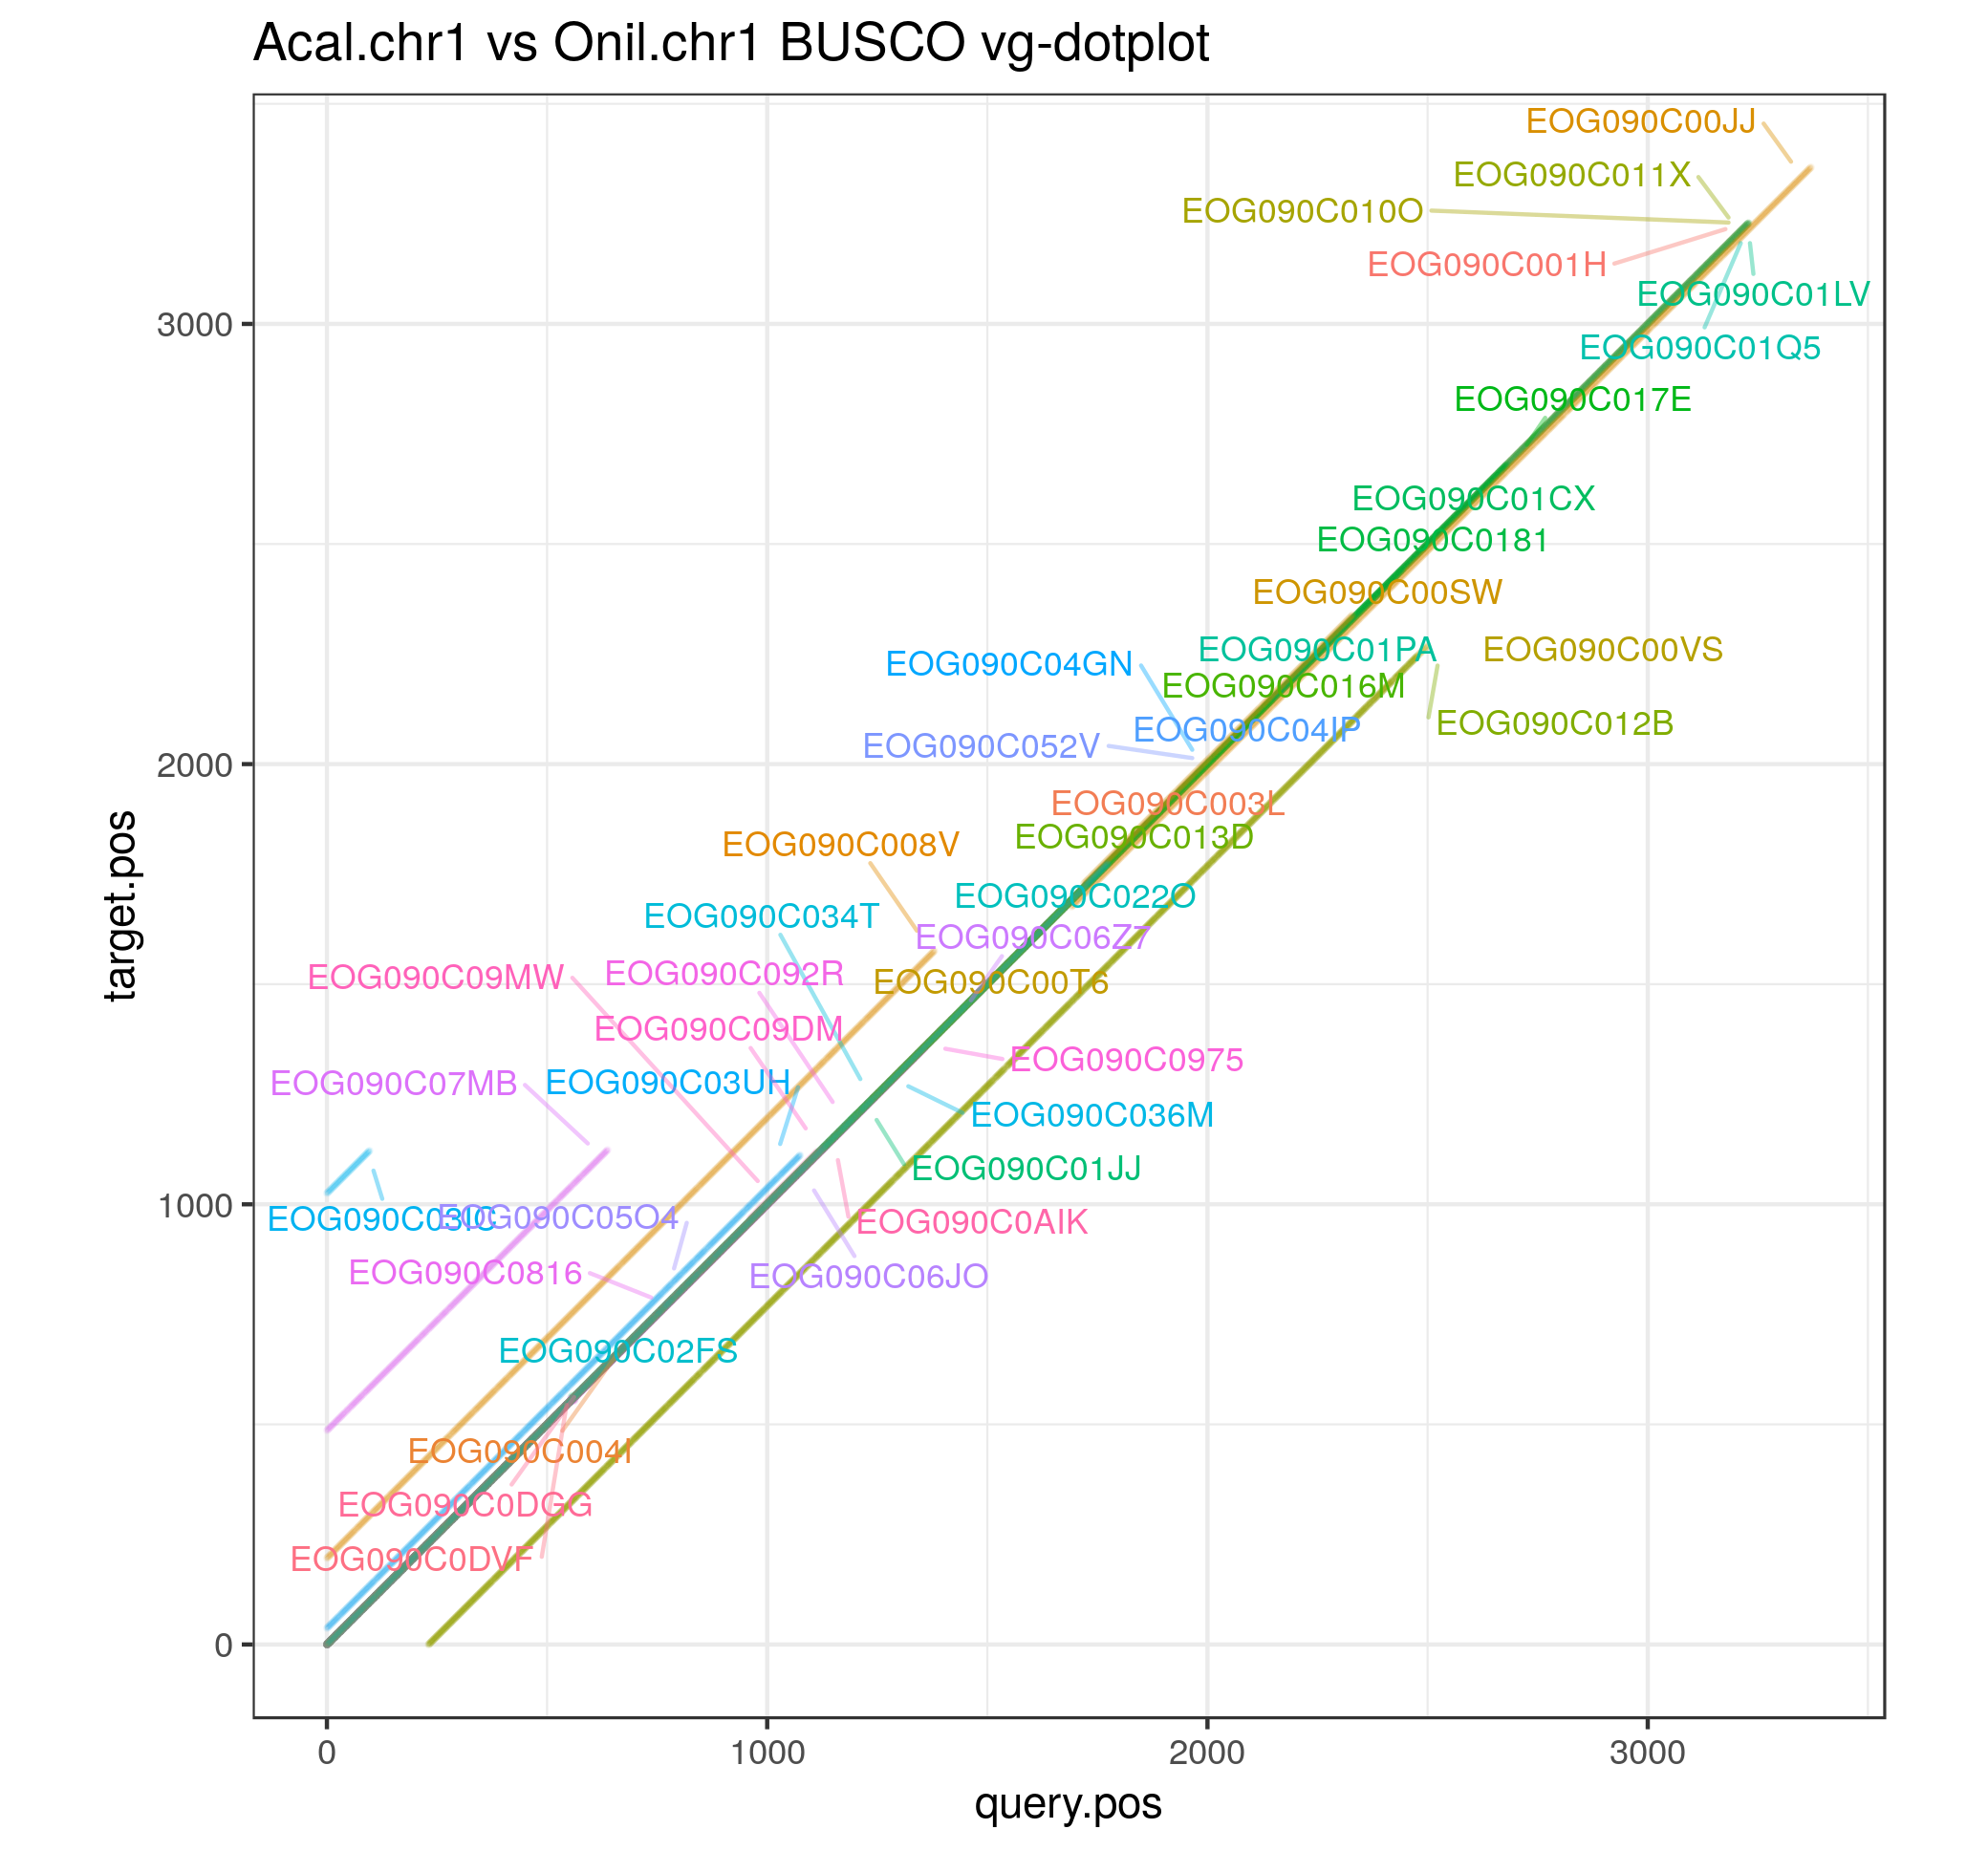
\includegraphics[scale=0.42,center]{cichlid_chr1_fpal10k_busco_dotplot_Acal_Onil.png}
  \end{figure}
\end{frame}

\begin{frame}
  \frametitle{BUSCO gene alignments from fpal10k graph, Acal vs Mzeb}
  \begin{figure}
    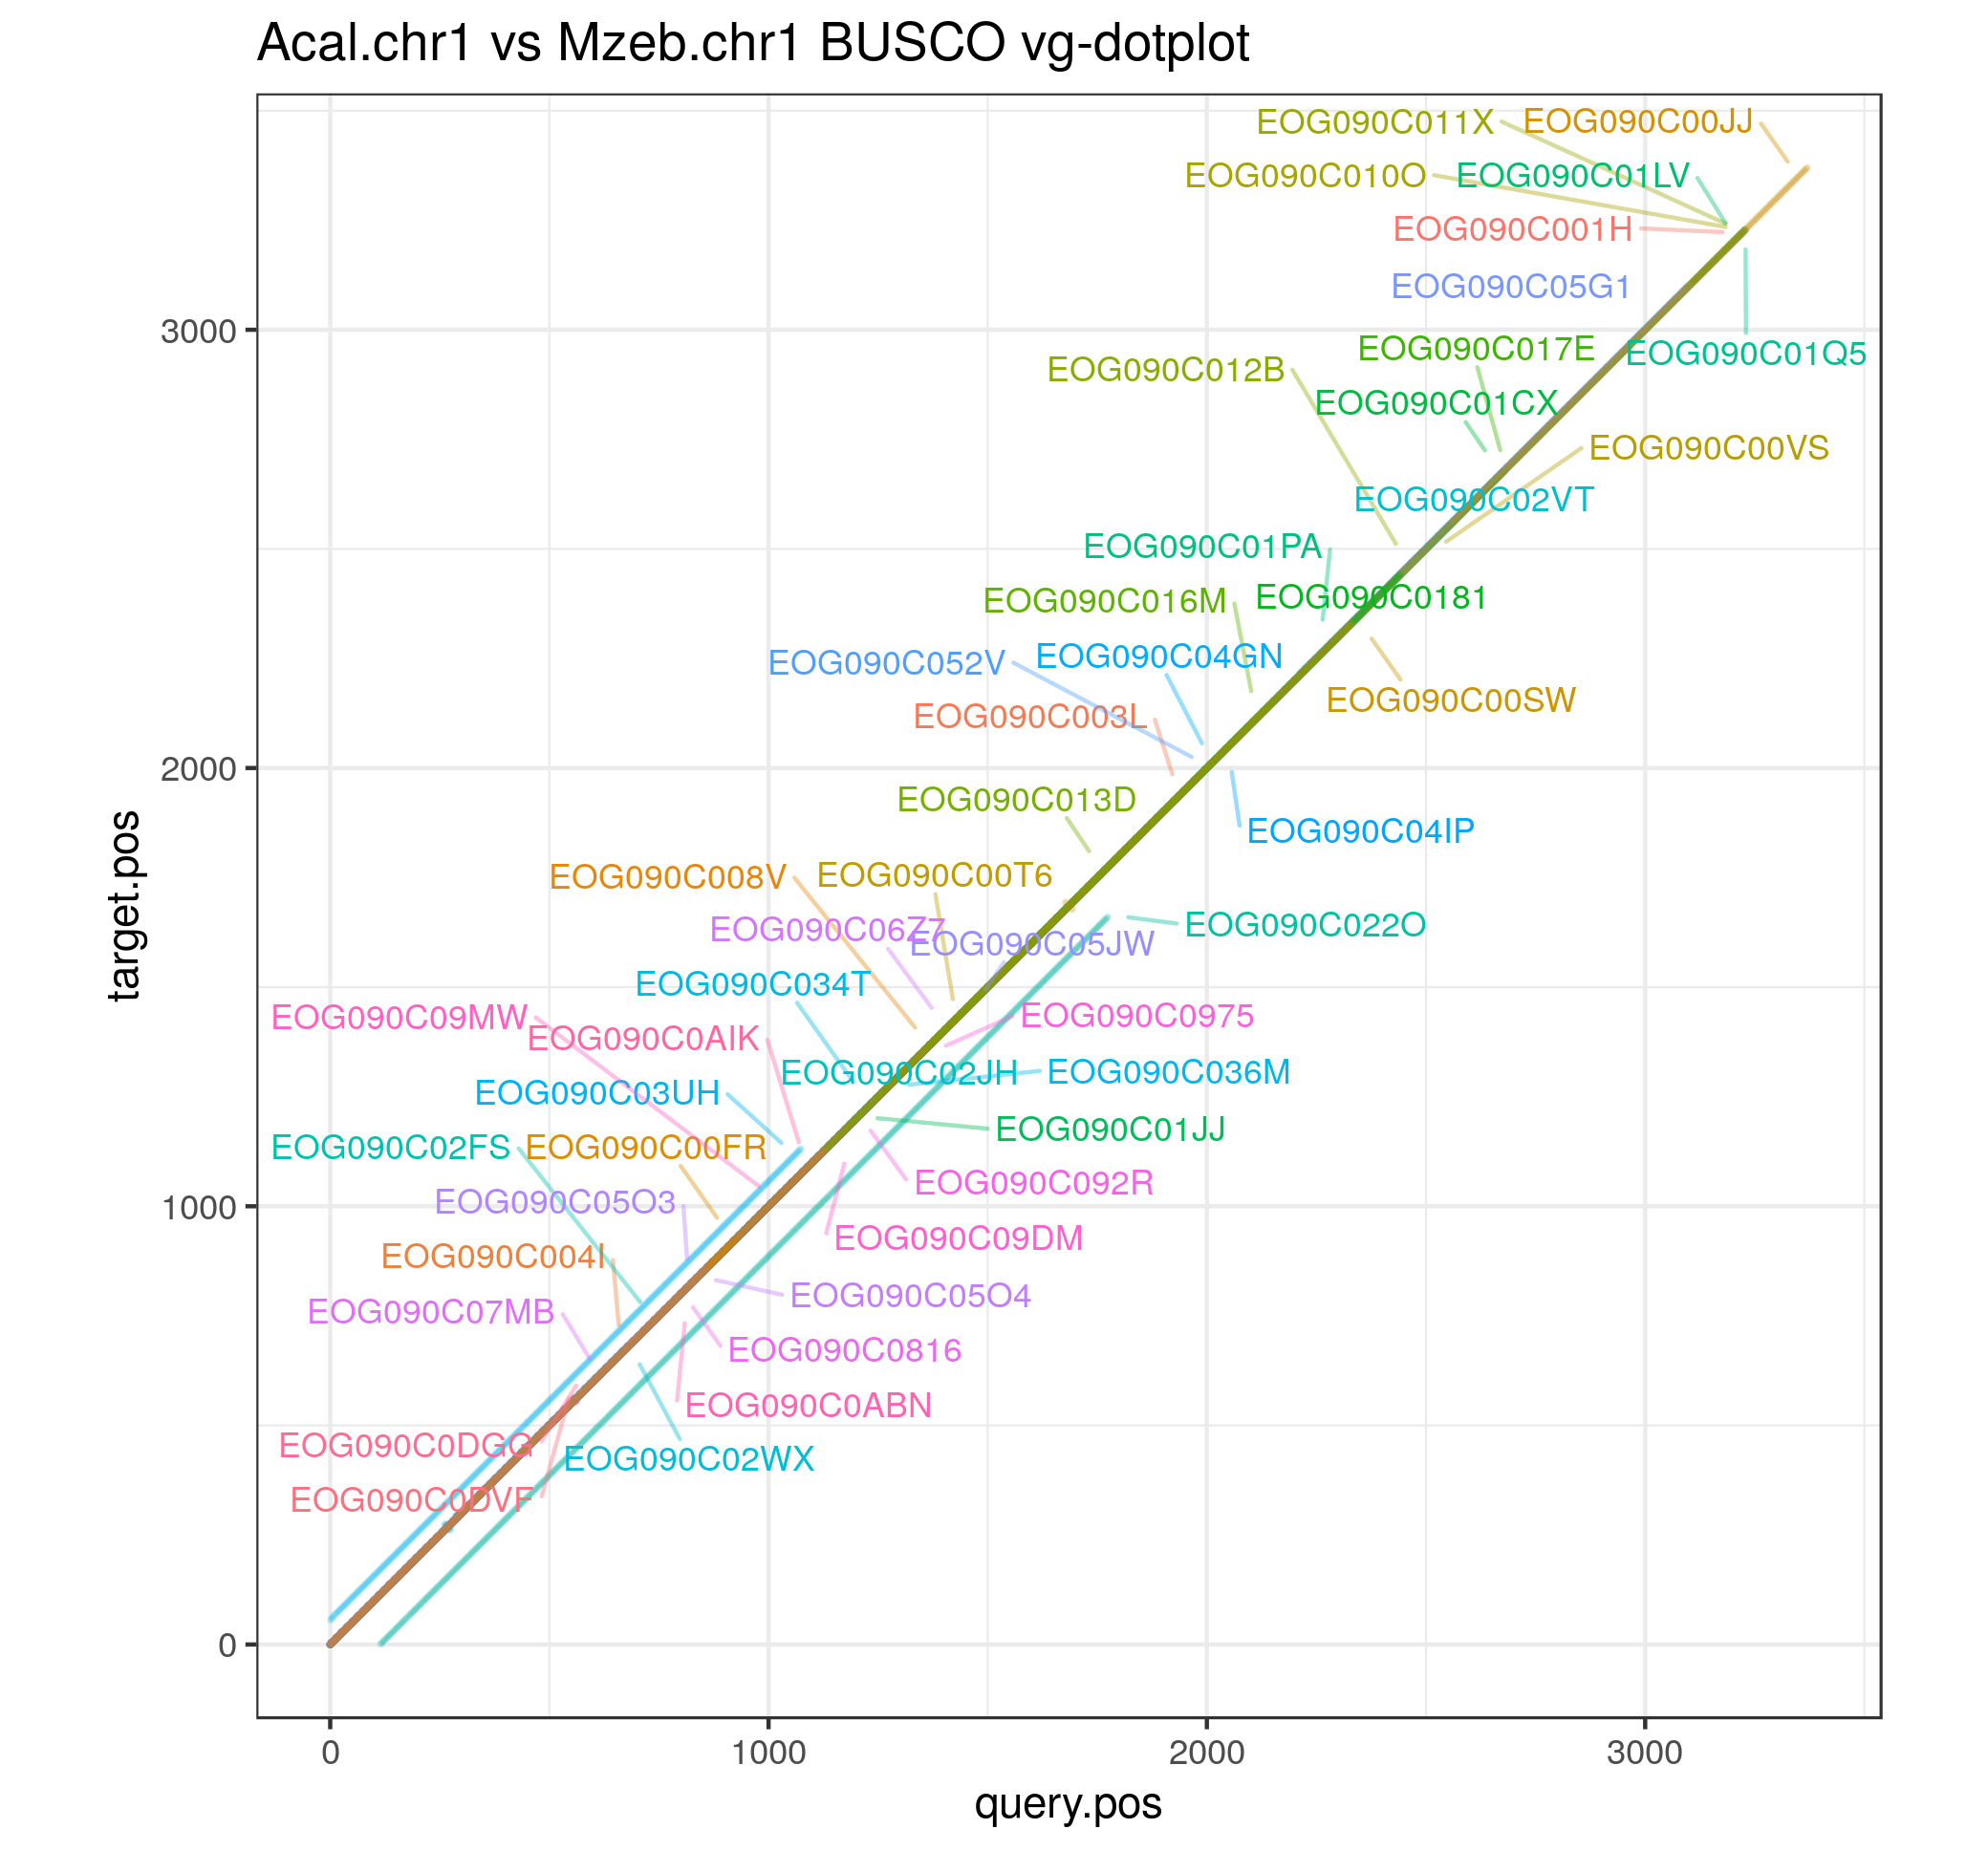
\includegraphics[scale=0.42,center]{cichlid_chr1_fpal10k_busco_dotplot_Acal_Mzeb.png}
  \end{figure}
\end{frame}

\begin{frame}
  \frametitle{BUSCO gene alignments from fpal10k graph, Mzeb vs Onil}
  \begin{figure}
    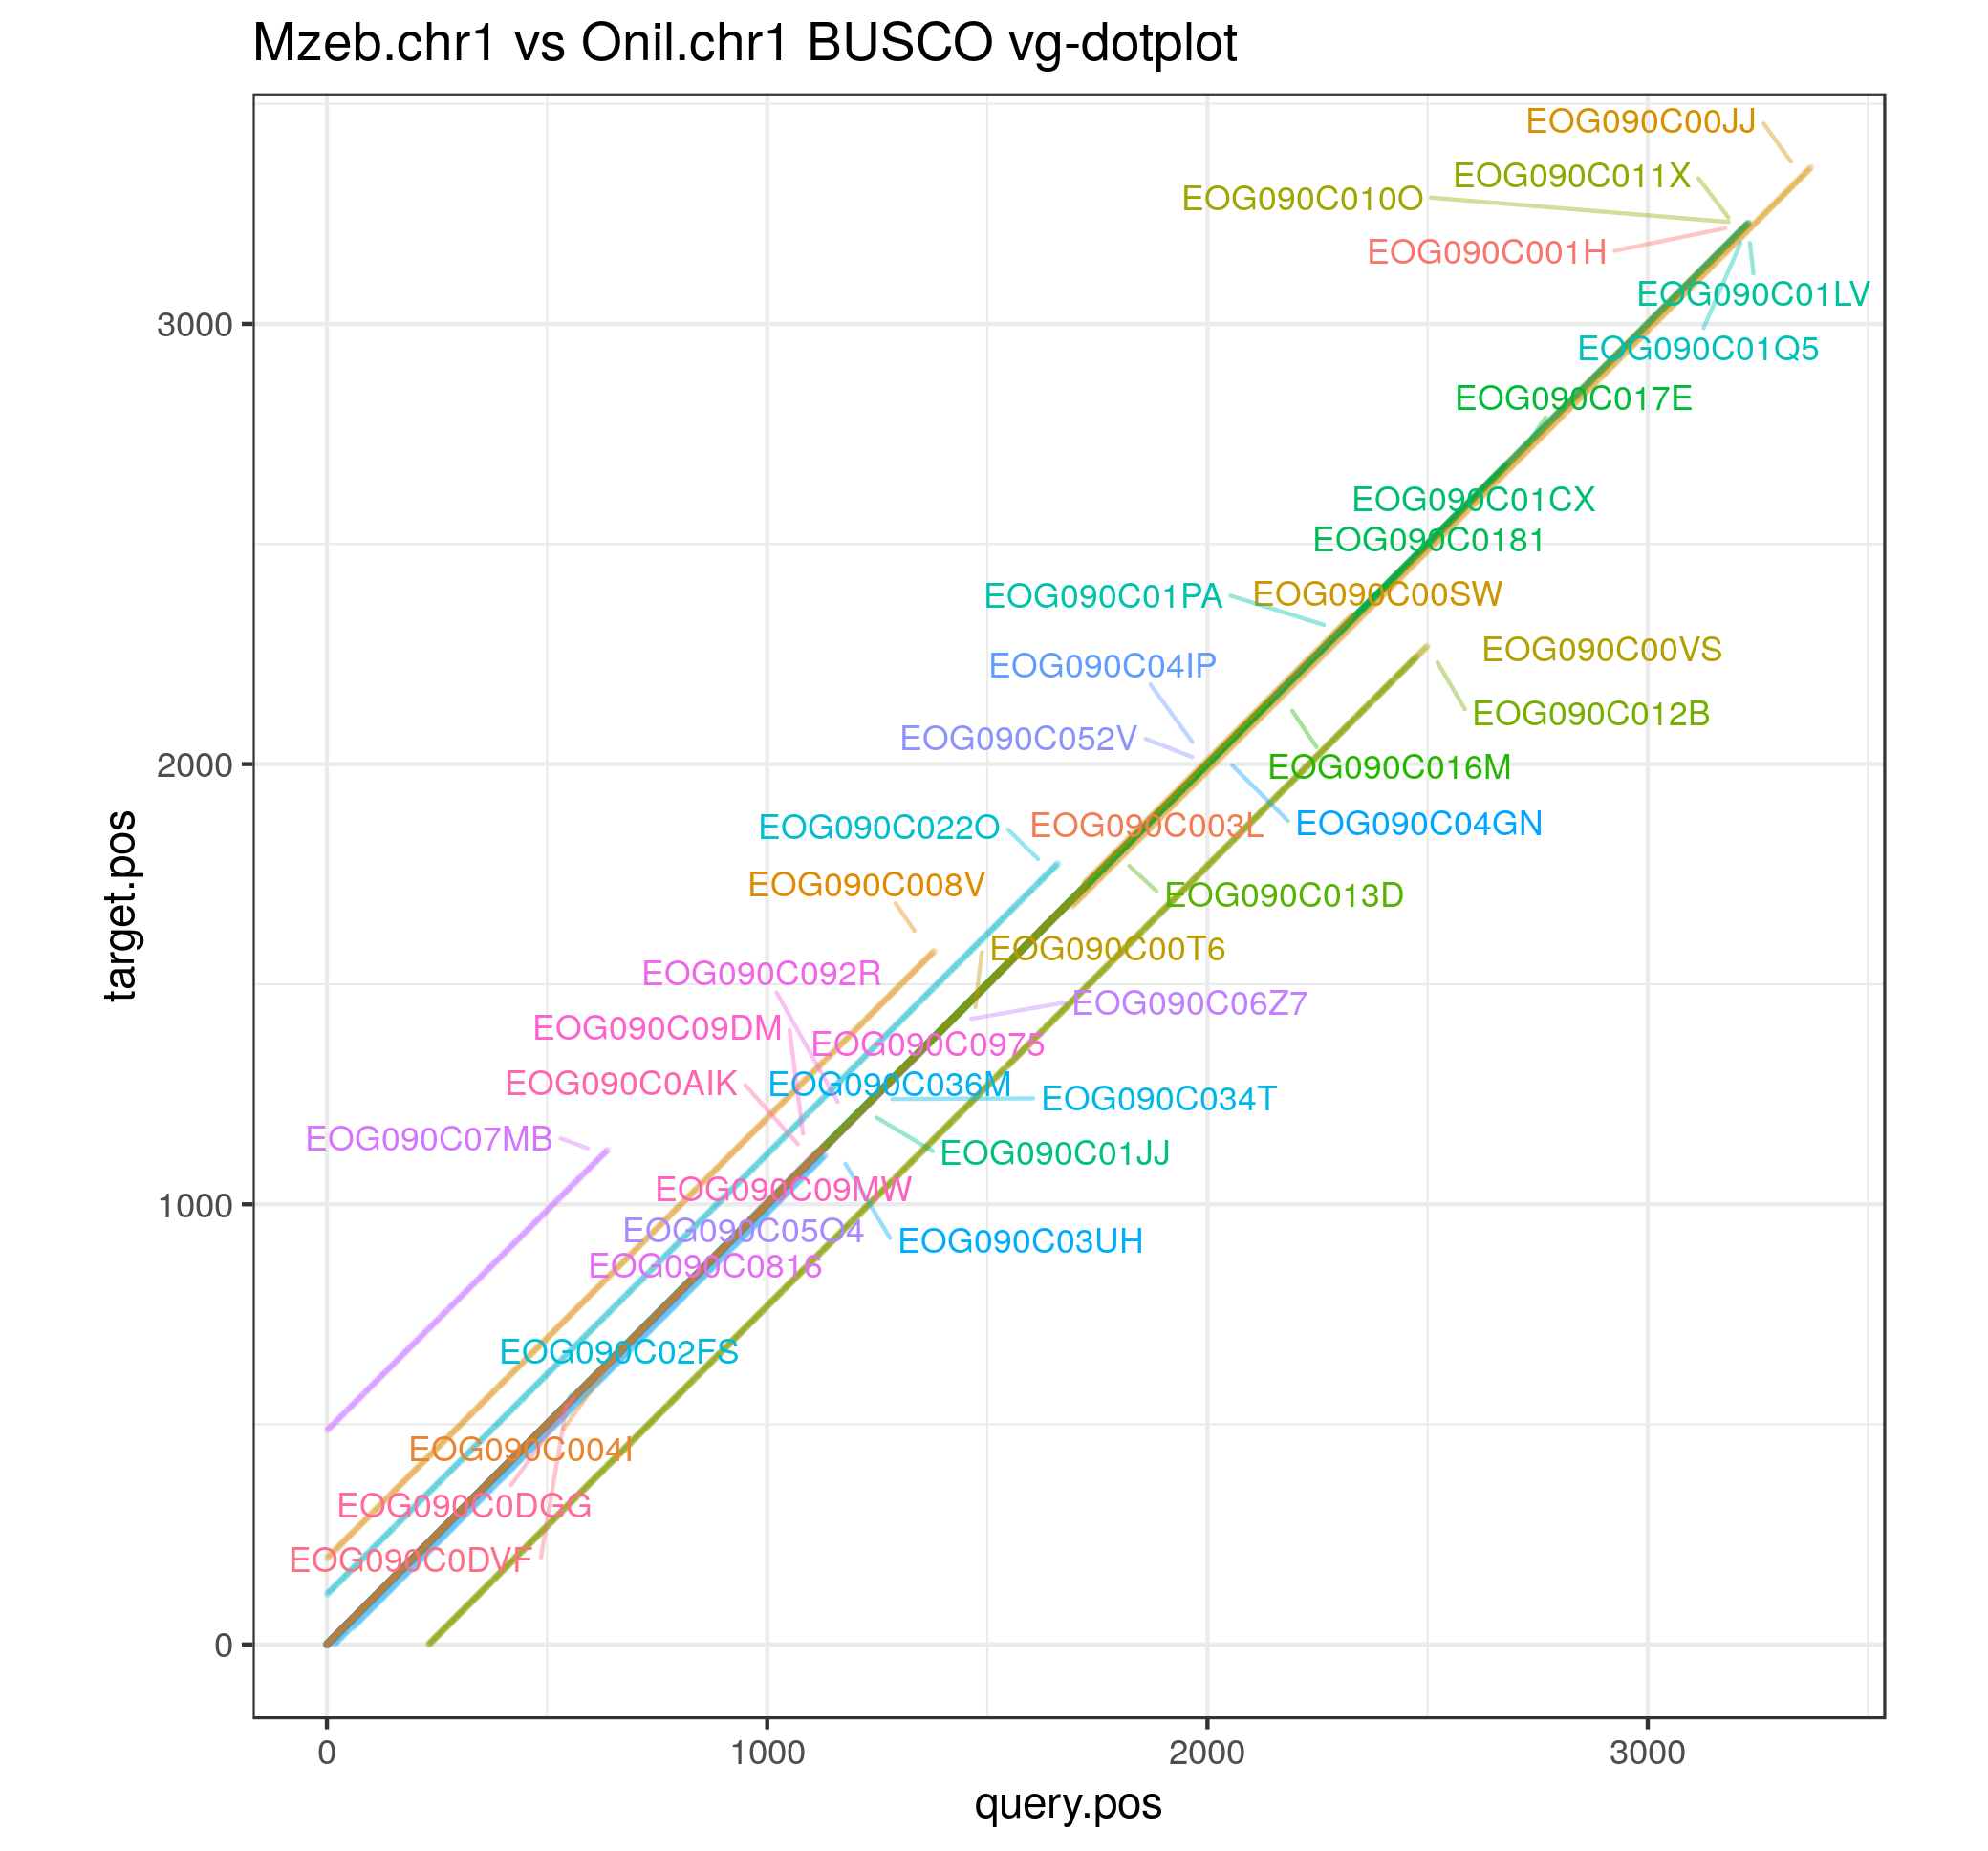
\includegraphics[scale=0.42,center]{cichlid_chr1_fpal10k_busco_dotplot_Mzeb_Onil.png}
  \end{figure}
\end{frame}

\begin{frame}[fragile]
  \frametitle{Absolute overlaps in fpal10k graph, Mzeb vs Onil}
    \begin{columns}[c] % The "c" option specifies centered vertical alignment while the "t" option is used for top vertical alignment
    \column{.35\textwidth} % Right column and width
    Using a tool that specifically checks for the in-graph overlaps between each pair of paths for a given gene.
\begin{verbatim}
Acal vs Mzeb     48     0.977
Acal vs Onil     48     0.802
Mzeb vs Onil     44     0.849
\end{verbatim}
\column{.45\textwidth} % Right column and width
    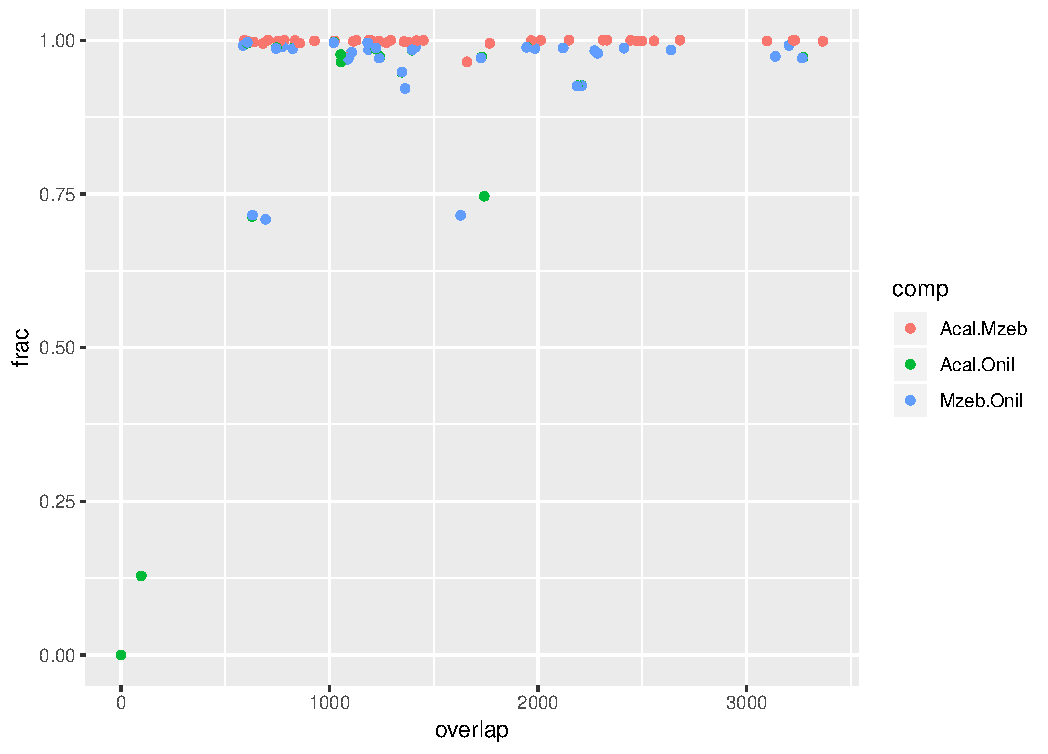
\includegraphics[scale=0.42,center]{busco-path-overlaps.pdf}
\end{columns}

\end{frame}

\section{Linear time whole genome alignment graph visualization}
\begin{frame}[fragile]
  \frametitle{Linear time genome graph visualization}
  The Bandage visualizations take many hours to produce, require dozens of gigabytes of RAM, and produce a result that isn't easy to interrogate.
  \\~\\
  In the past, I've worked on linear visualization of graphs.
  However, these are based in vector graphics and thus not scalable.
  \begin{figure}
    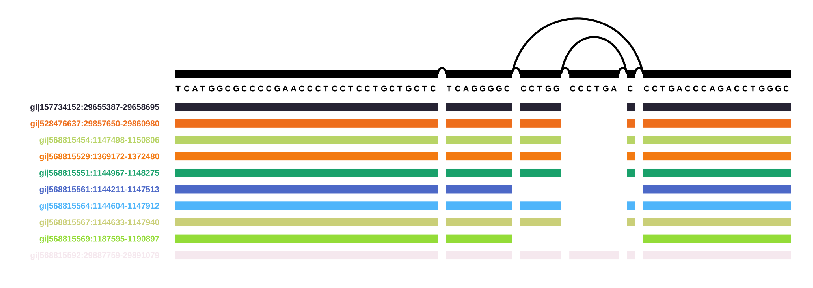
\includegraphics[scale=1,center]{vg_viz_H-3136_crop.pdf}
  \end{figure}
\end{frame}


\begin{frame}[fragile]
  \frametitle{\emph{Aggregated} linear time genome graph visualization}
  By directly aggregating the visualization into an image buffer, it's possible to achive very scalable visualizations of whole genome graphs \emph{that include path information} and provide insight into the structure of the graph.
\end{frame}

\begin{frame}[fragile]
  \frametitle{DRB1-3123 seqwish}
  \begin{figure}
    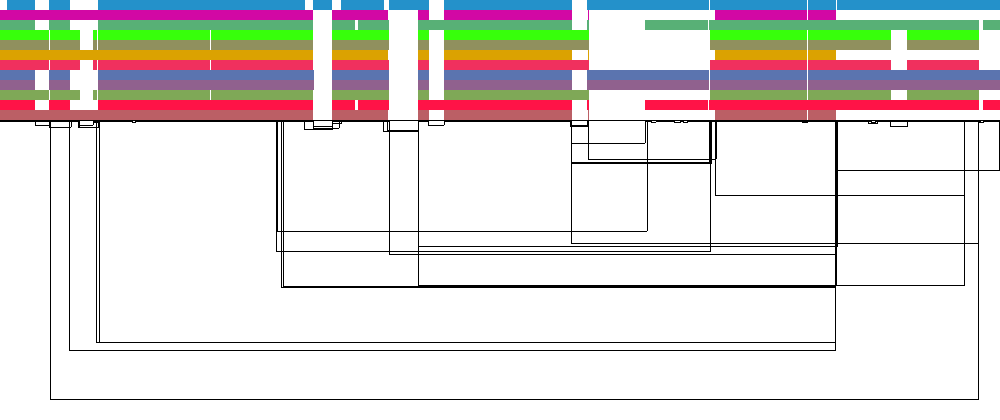
\includegraphics[scale=0.4,center]{DRB1-3123-seqwish-dg.png}
  \end{figure}
  This can give us insight into the differences between graphs.
\end{frame}

\begin{frame}[fragile]
  \frametitle{DRB1-3123 vg msga}
  \begin{figure}
    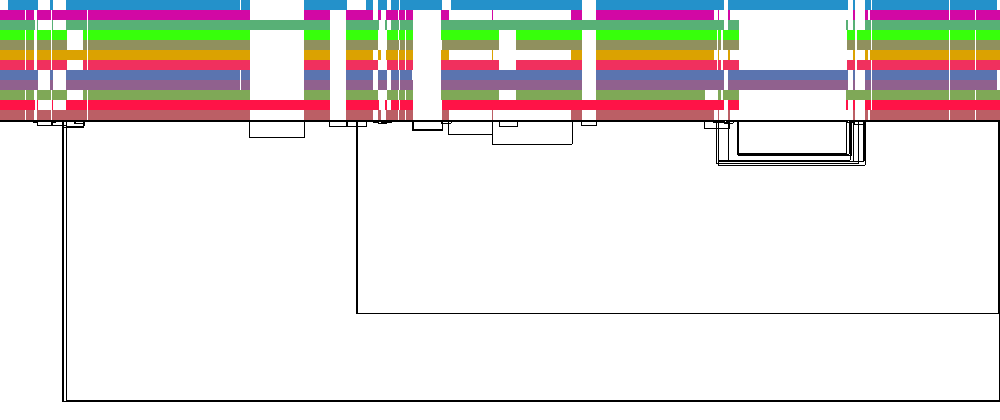
\includegraphics[scale=0.4,center]{DRB1-3123-vg-dg.png}
  \end{figure}
  This can give us insight into the differences between graphs.
\end{frame}

\begin{frame}[fragile]
  \frametitle{Cichlid chr1 graph, no filters}
  \begin{figure}
    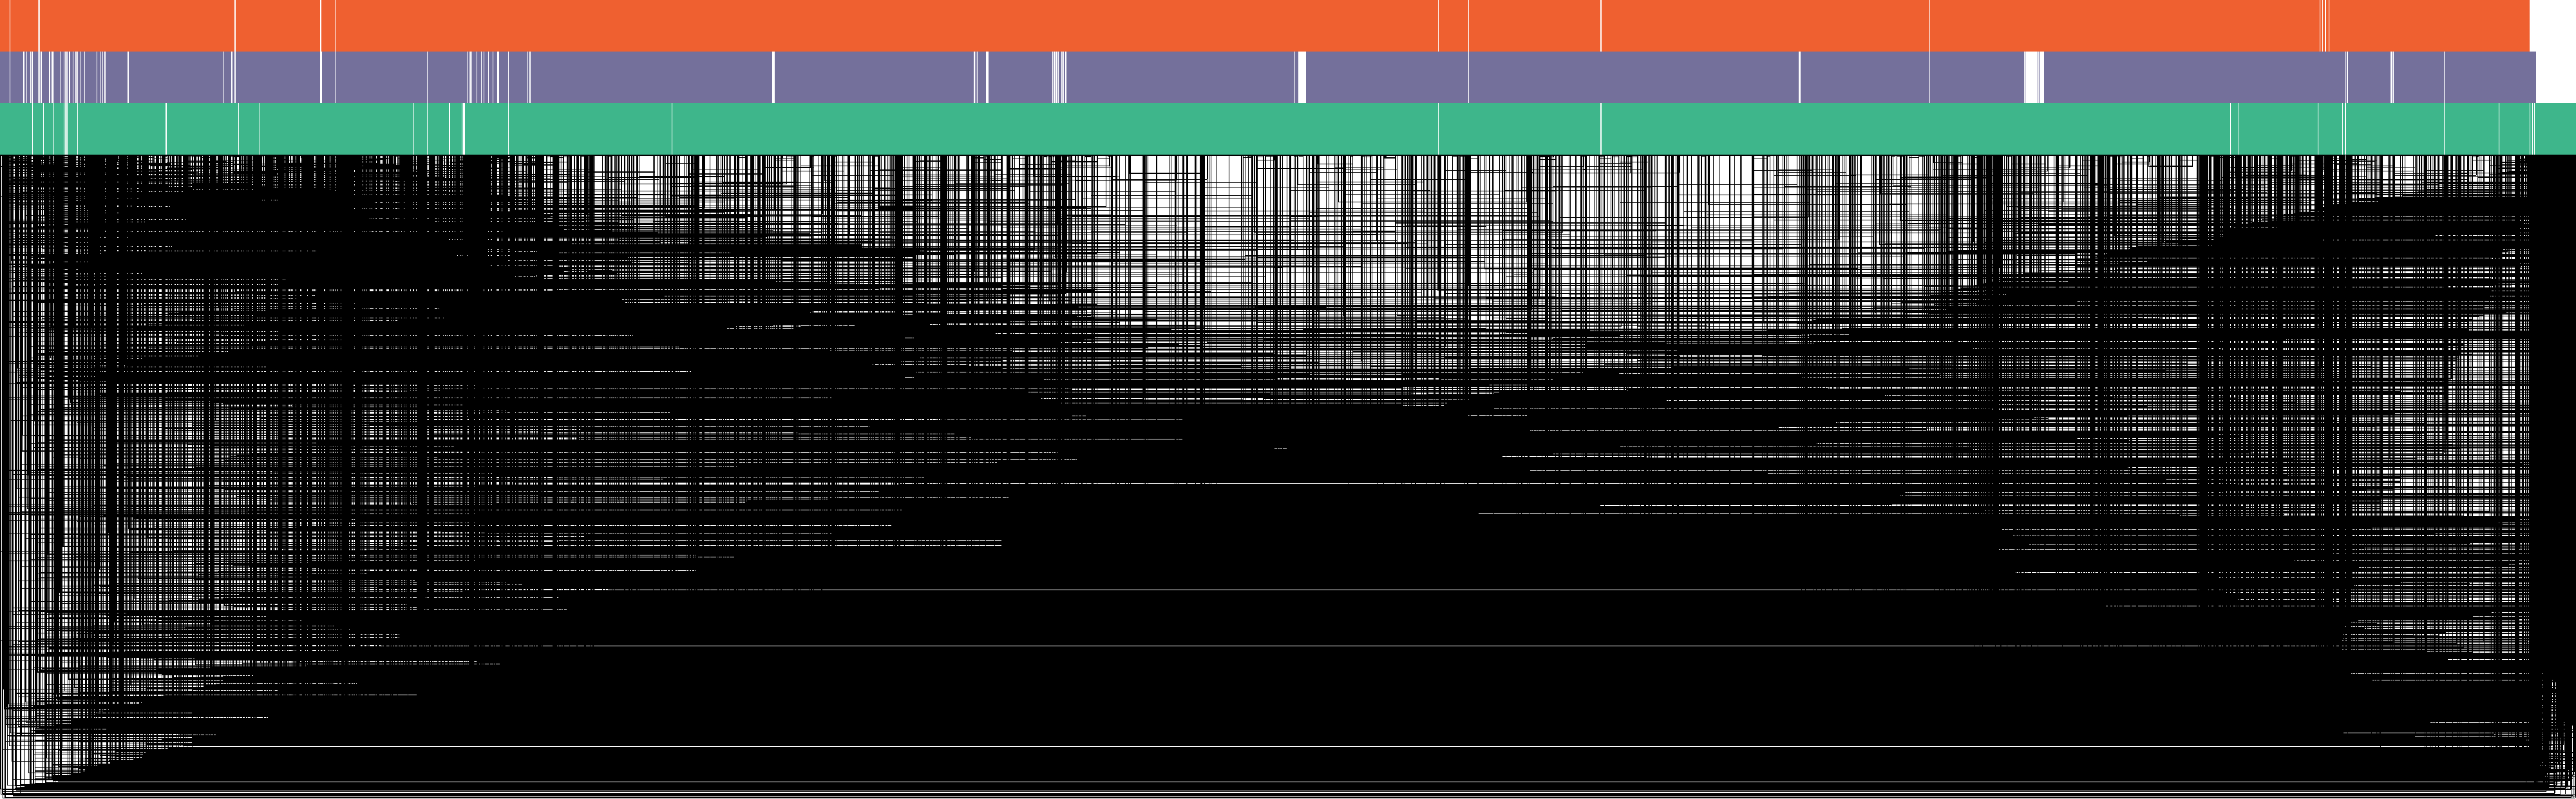
\includegraphics[scale=0.11,center]{cichlid-chr1-dg.png}
  \end{figure}
\end{frame}

\begin{frame}[fragile]
  \frametitle{Cichlid chr1 graph, fpa -l 2k}
  \begin{figure}
    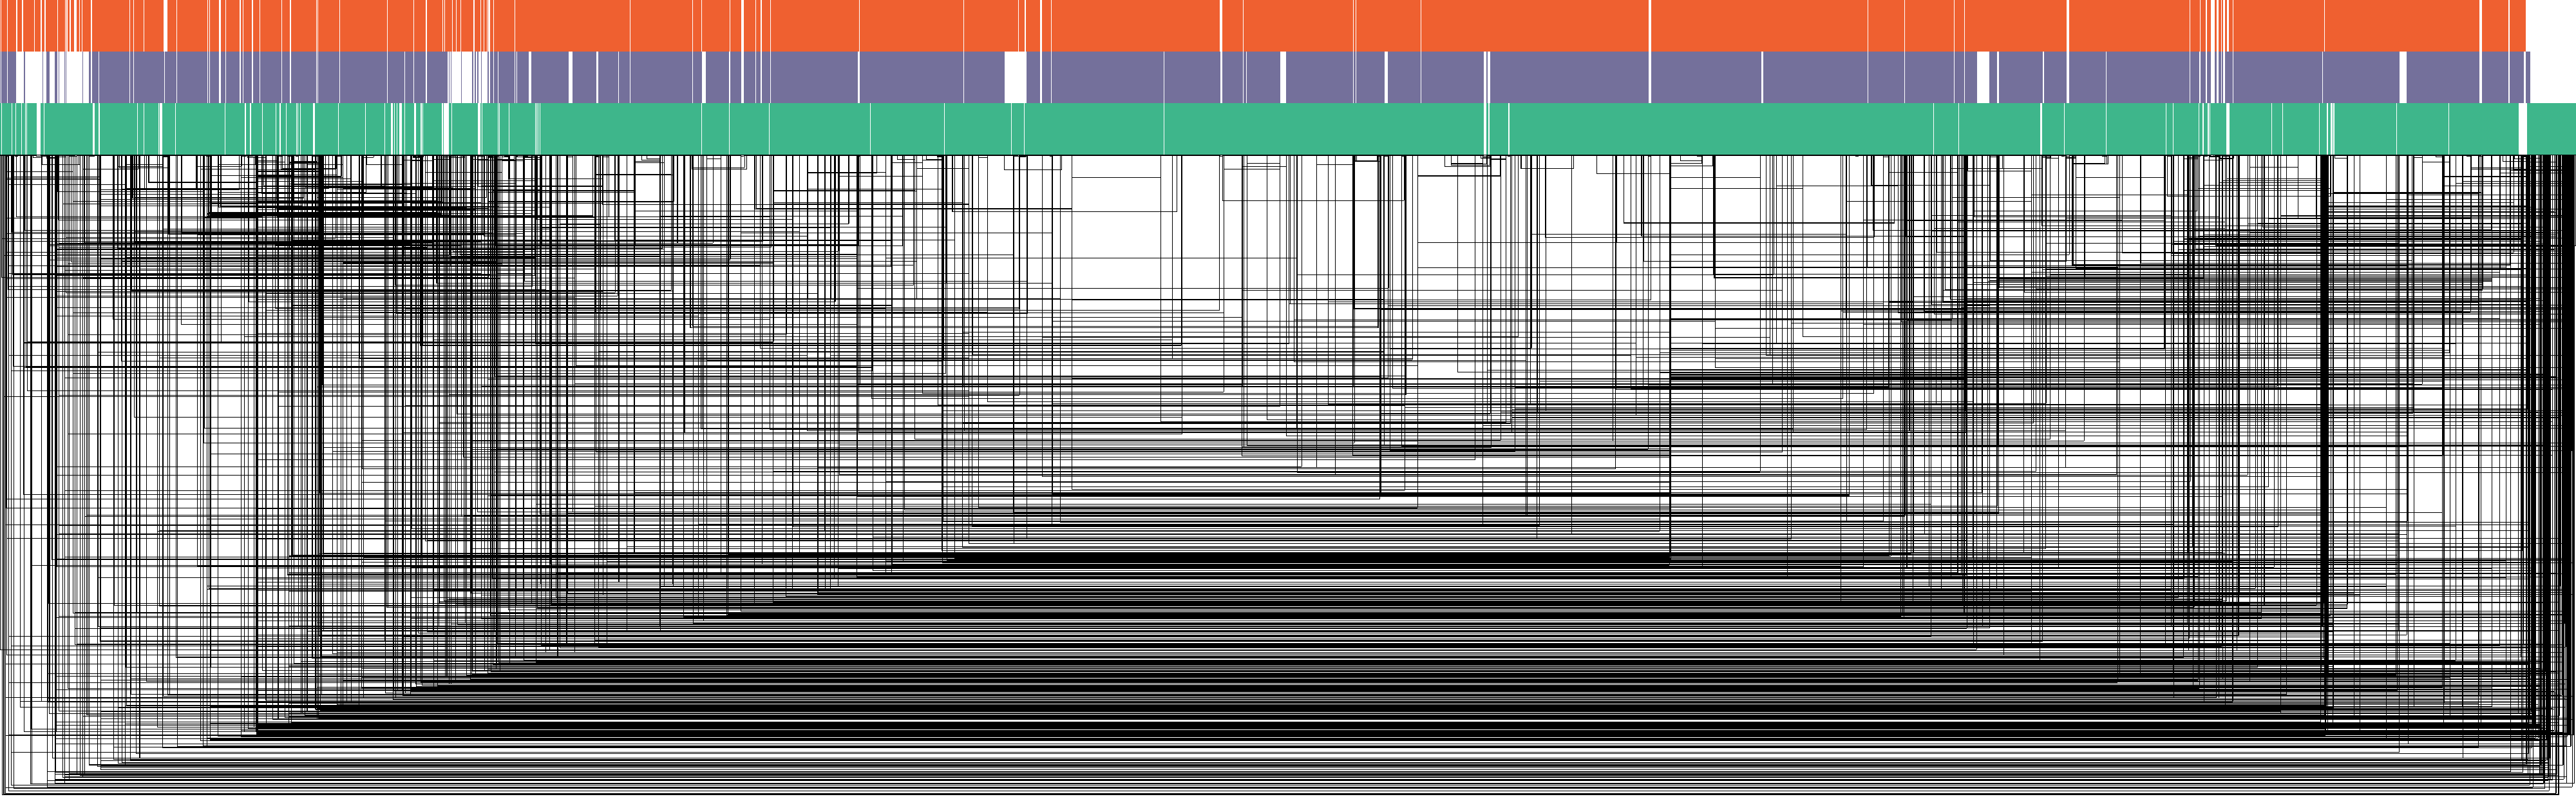
\includegraphics[scale=0.11,center]{cichlid-chr1-fpal2k-dg.png}
  \end{figure}
\end{frame}

\begin{frame}[fragile]
  \frametitle{Cichlid chr1 graph, fpa -l 10k}
  \begin{figure}
    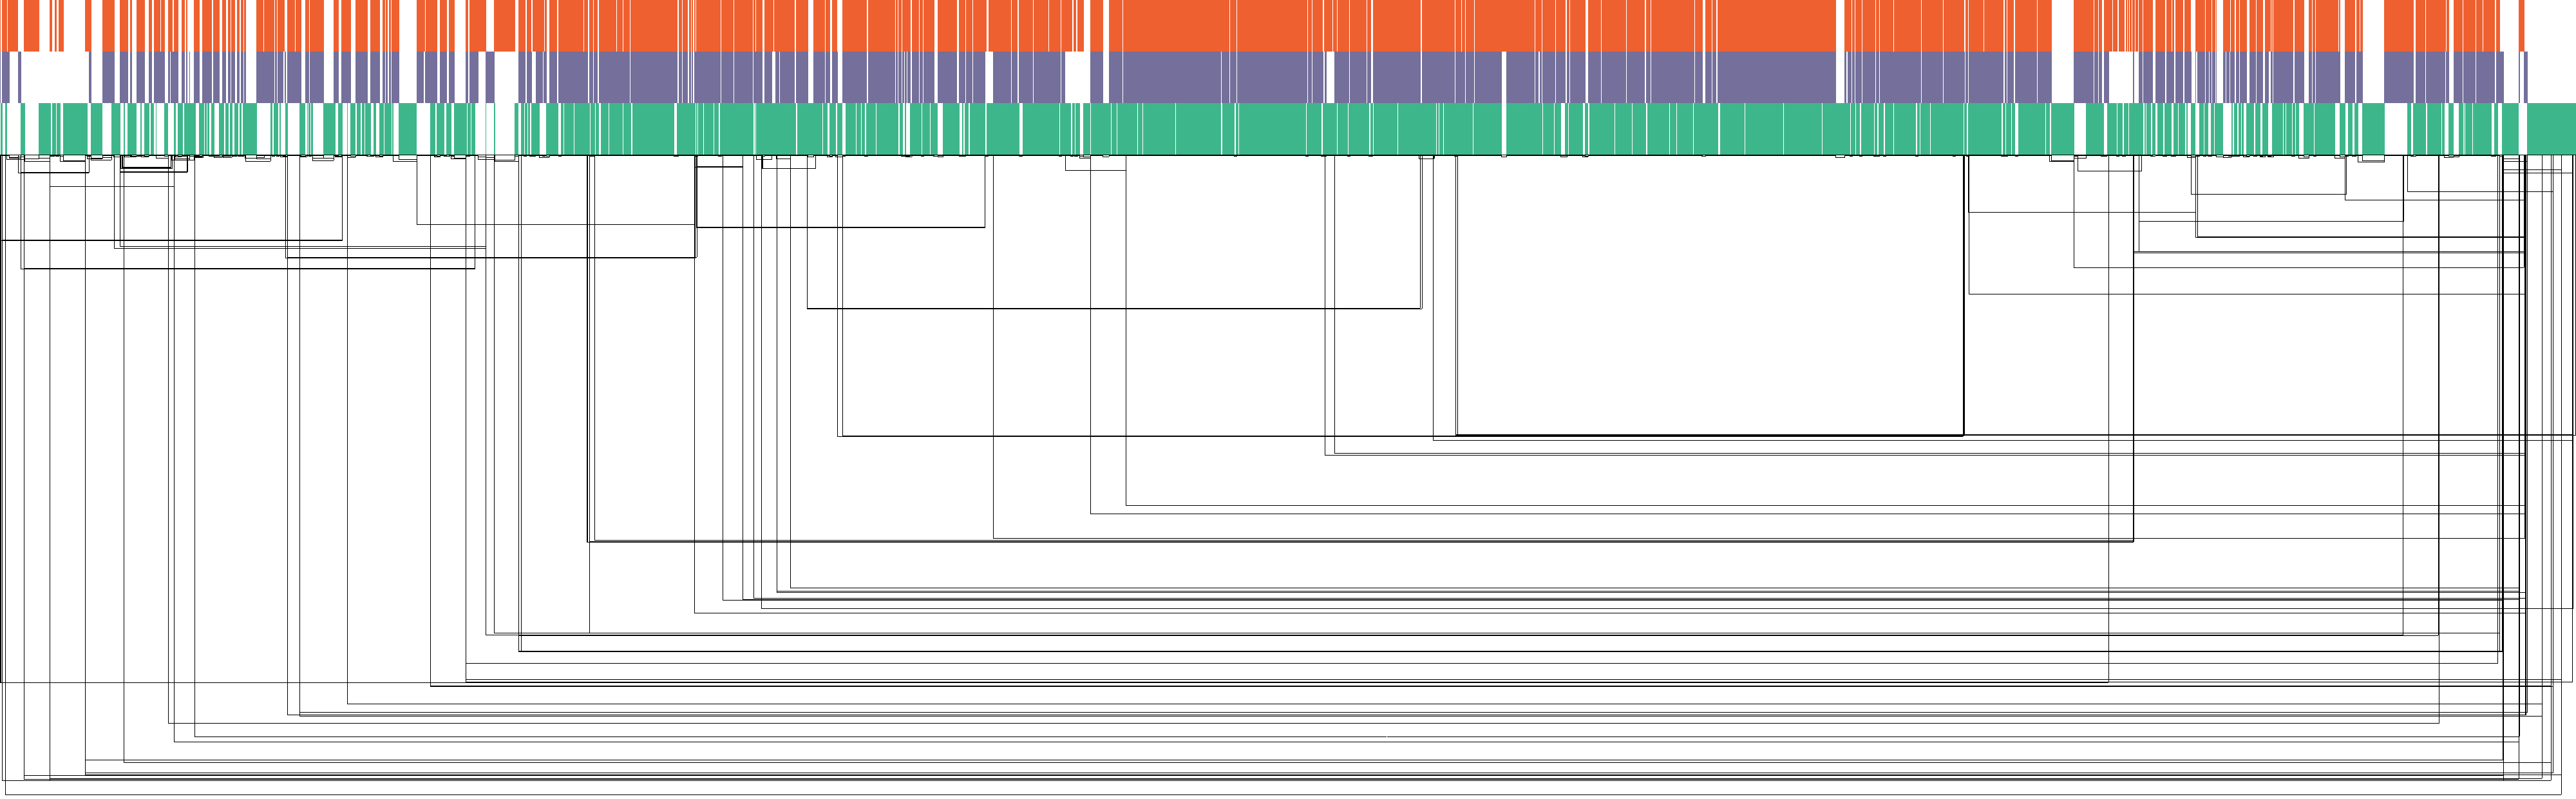
\includegraphics[scale=0.11,center]{cichlid-chr1-fpal10k-dg.png}
  \end{figure}
\end{frame}

\begin{frame}[fragile]
  \frametitle{Cichlid chr1 graph, fpa -l 20k}
  \begin{figure}
    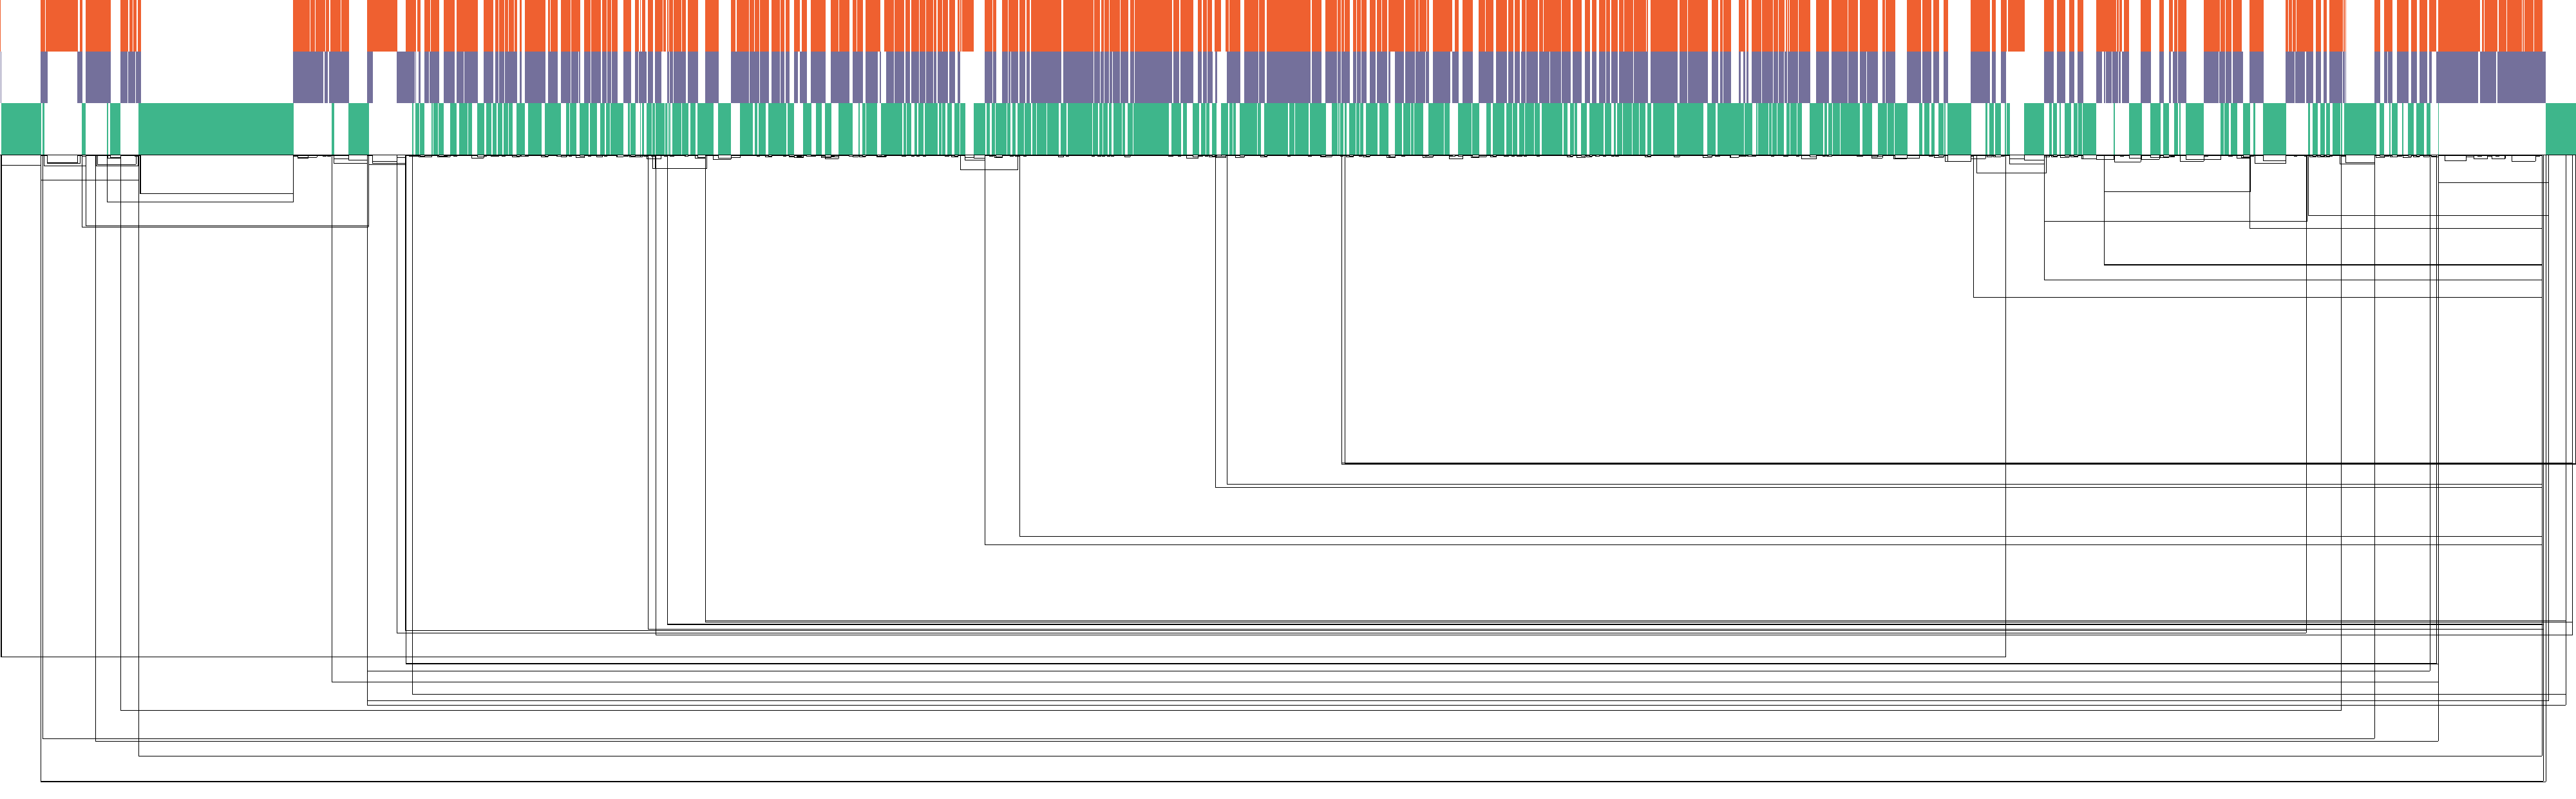
\includegraphics[scale=0.11,center]{cichlid-chr1-fpal20k-dg.png}
  \end{figure}
\end{frame}

\begin{frame}[fragile]
  \frametitle{Cichlid chr1 graph, fpa -l 50k}
  \begin{figure}
    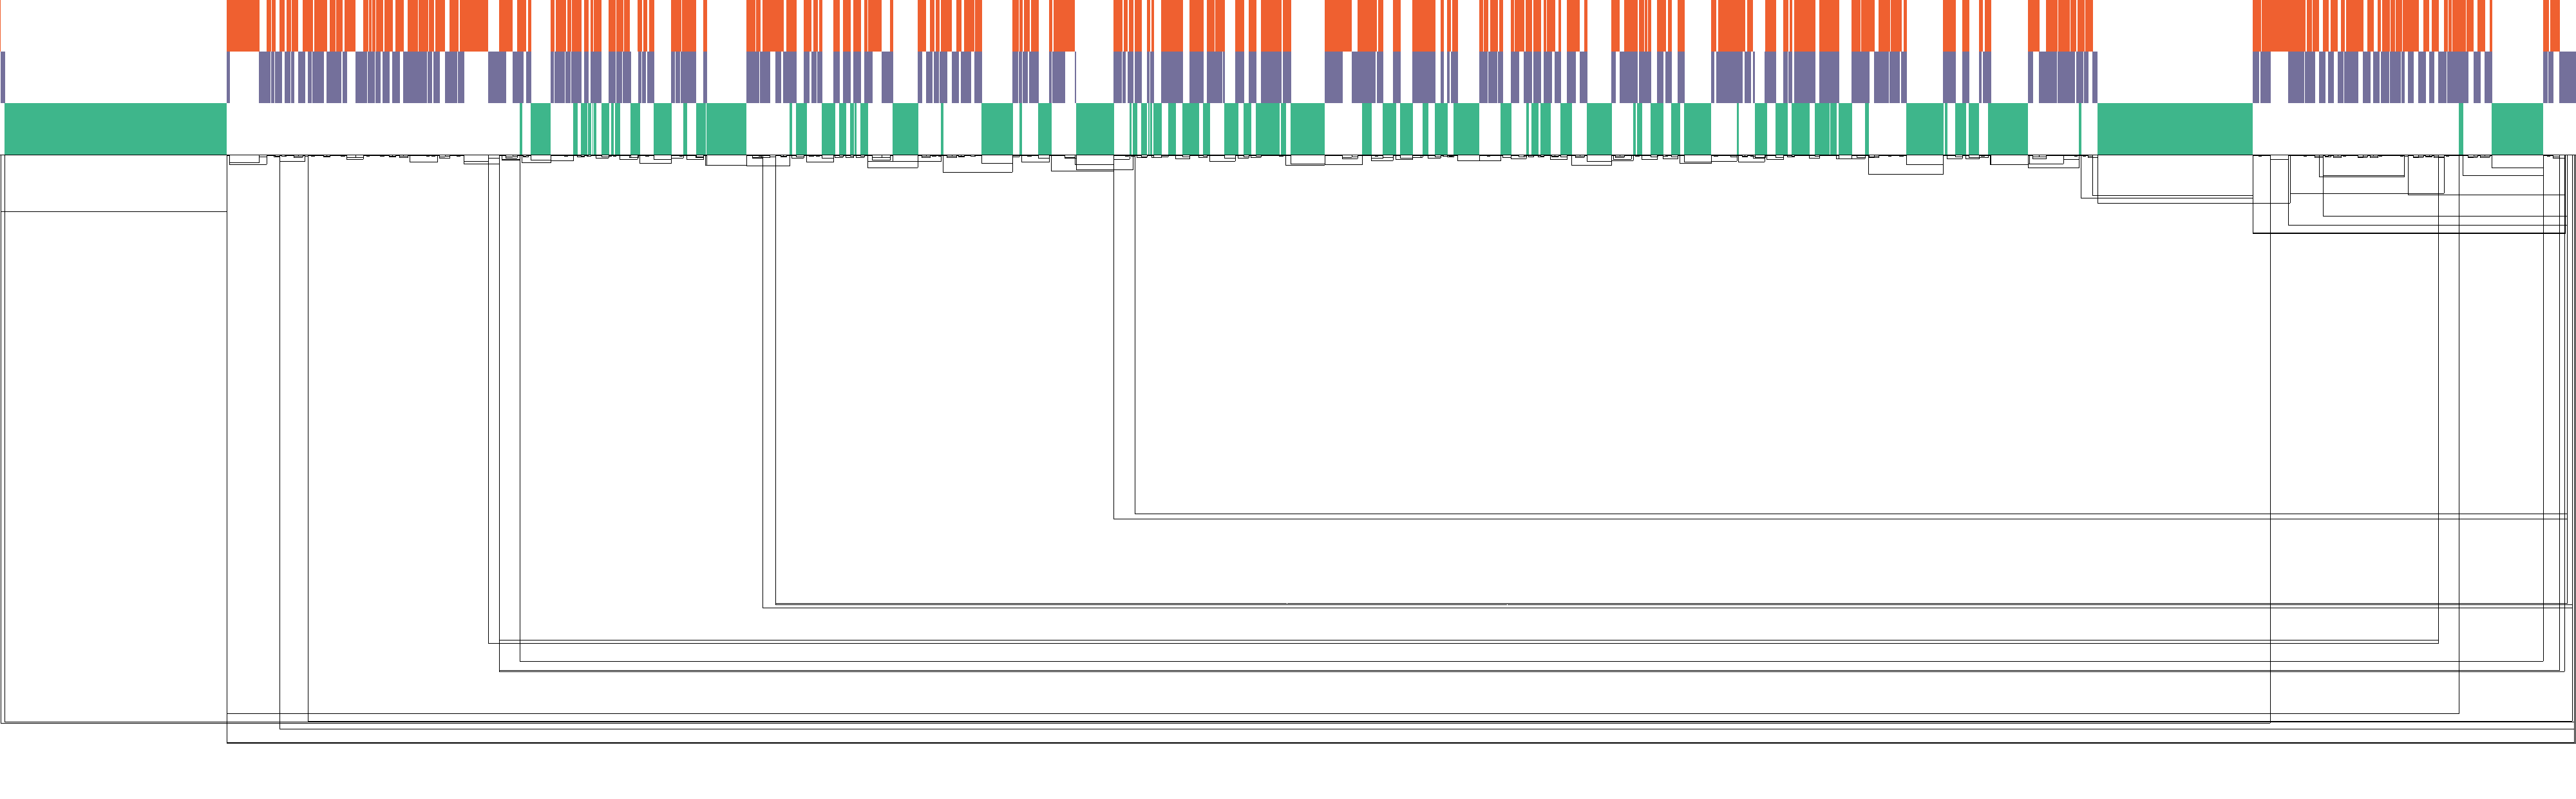
\includegraphics[scale=0.11,center]{cichlid-chr1-fpal50k-dg.png}
  \end{figure}
\end{frame}


\begin{frame}[fragile]
  \frametitle{Yue 2016 yeast strains, Cactus alignment}
  \begin{figure}
    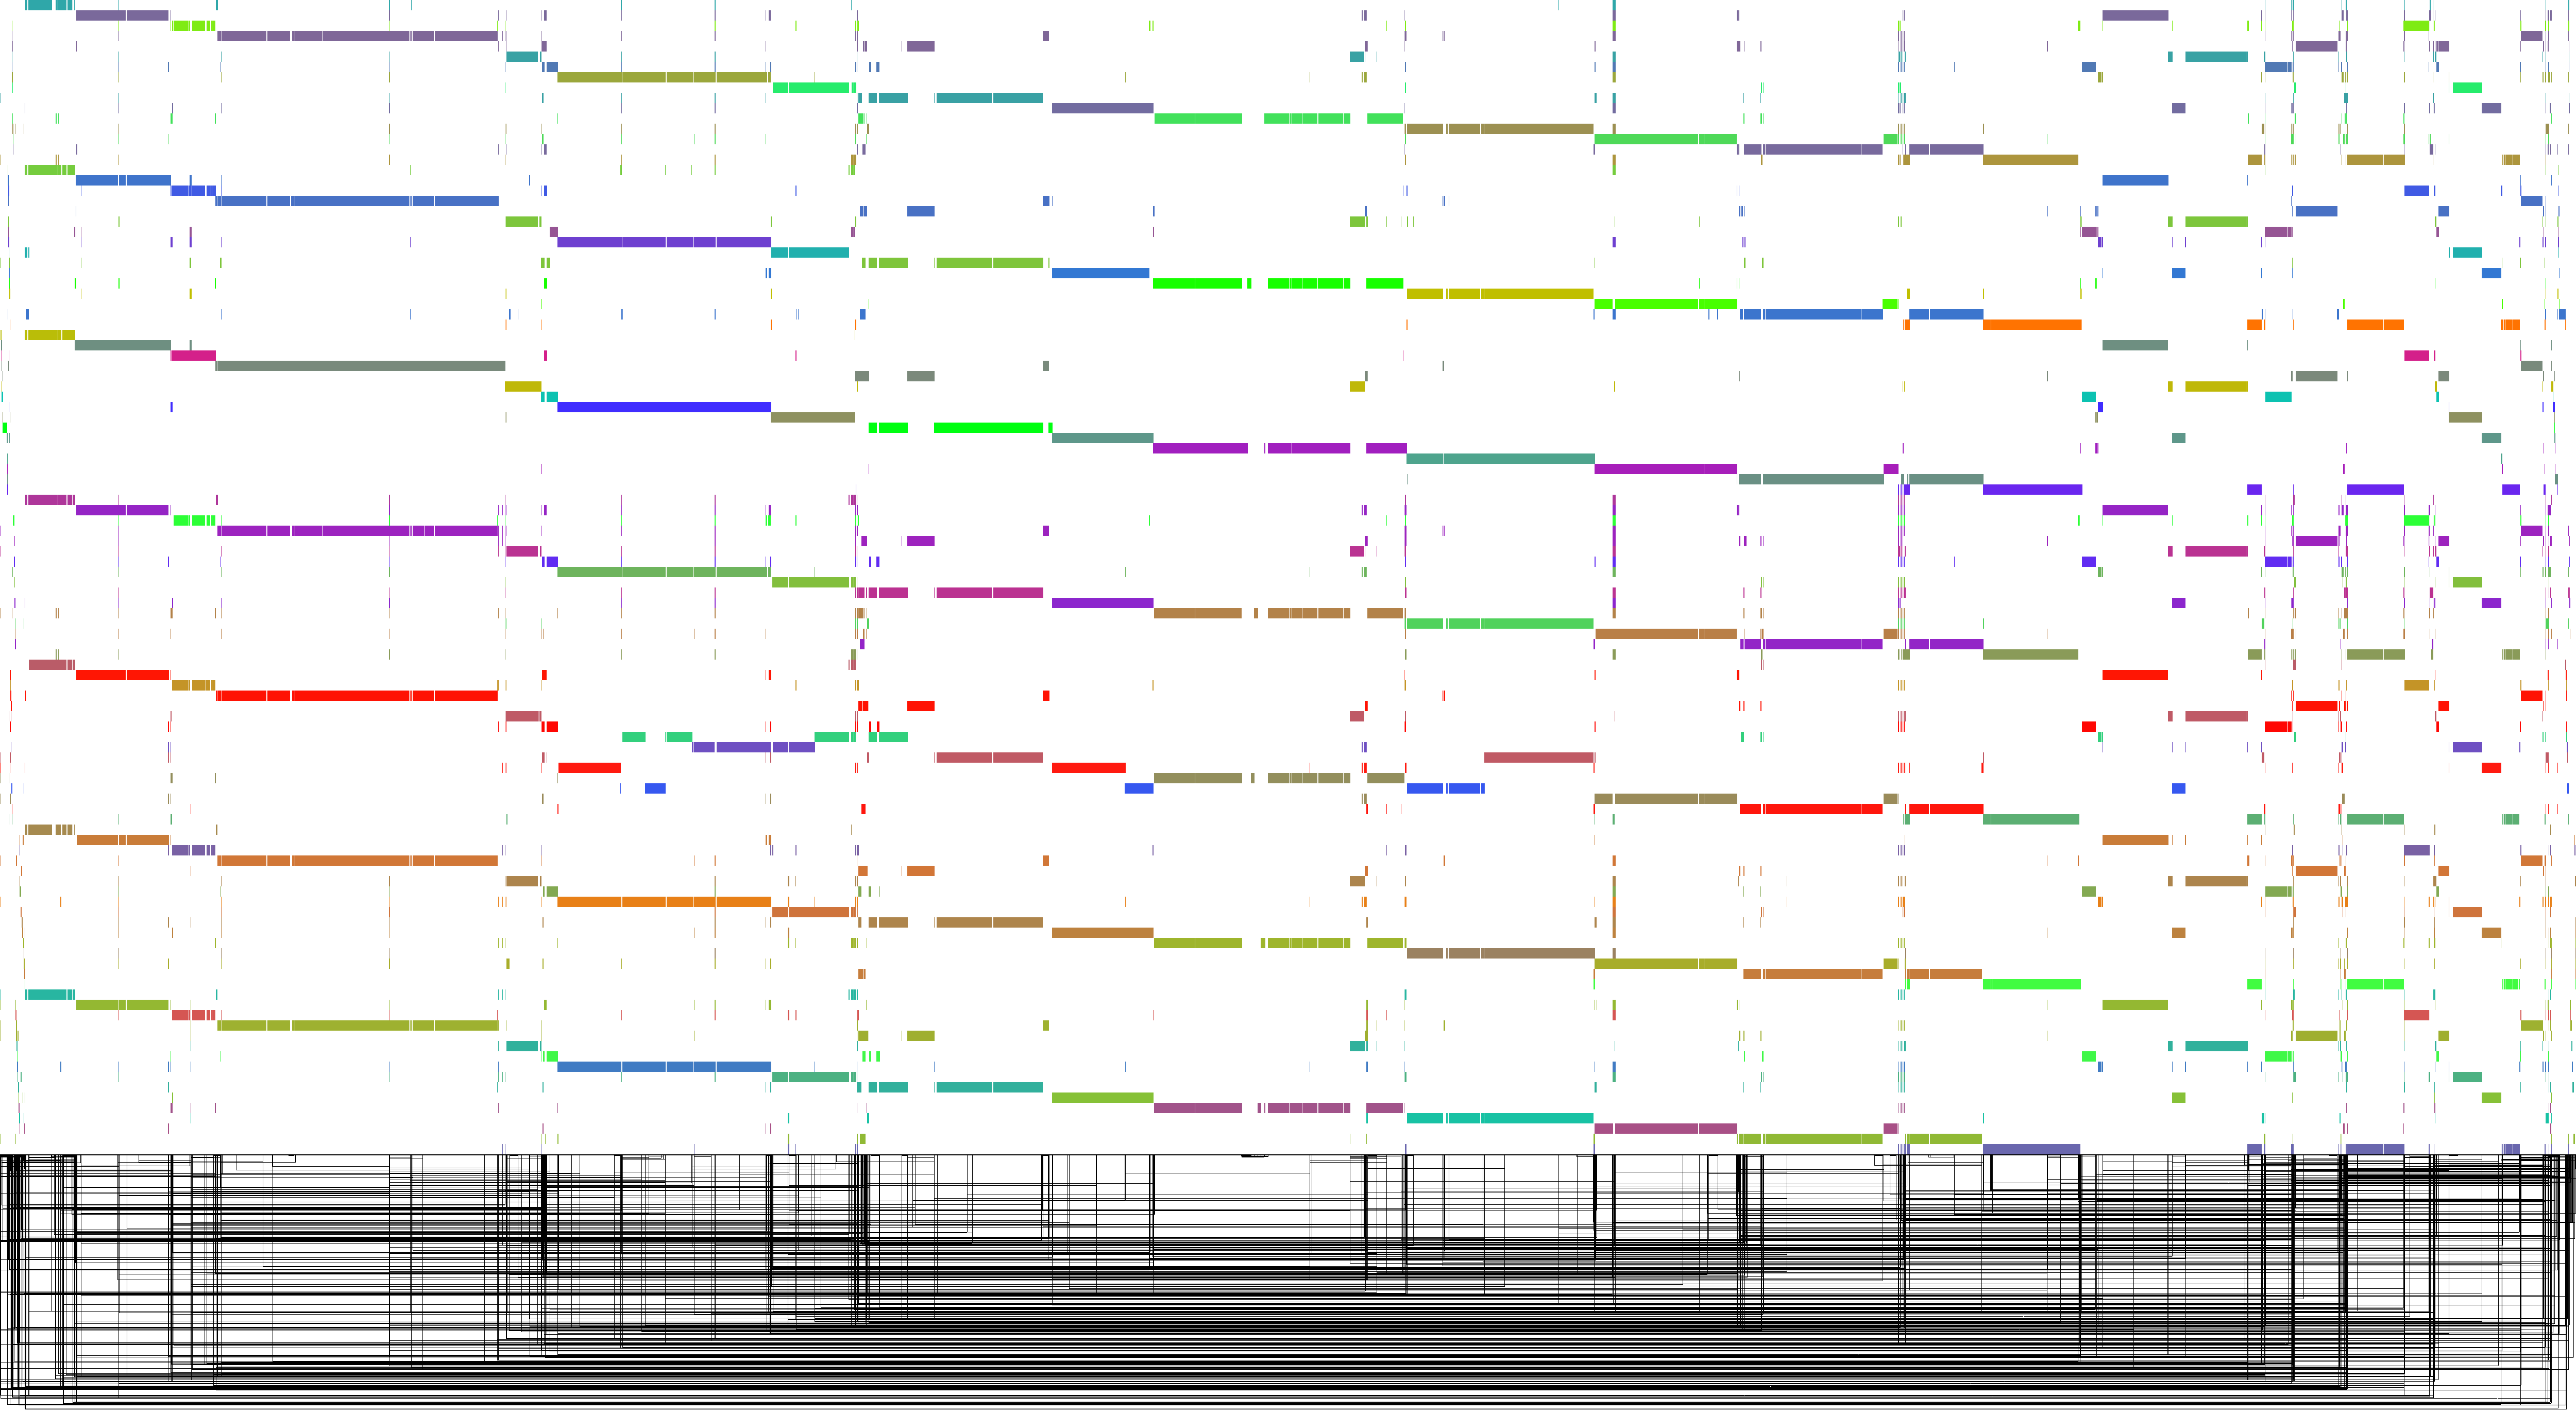
\includegraphics[scale=0.08,center]{cactus-yeast-dg.png}
  \end{figure}
\end{frame}

\begin{frame}[fragile]
  \frametitle{Yue 2016 yeast strains, Seqwish (10kb filtered) alignment}
  \begin{figure}
    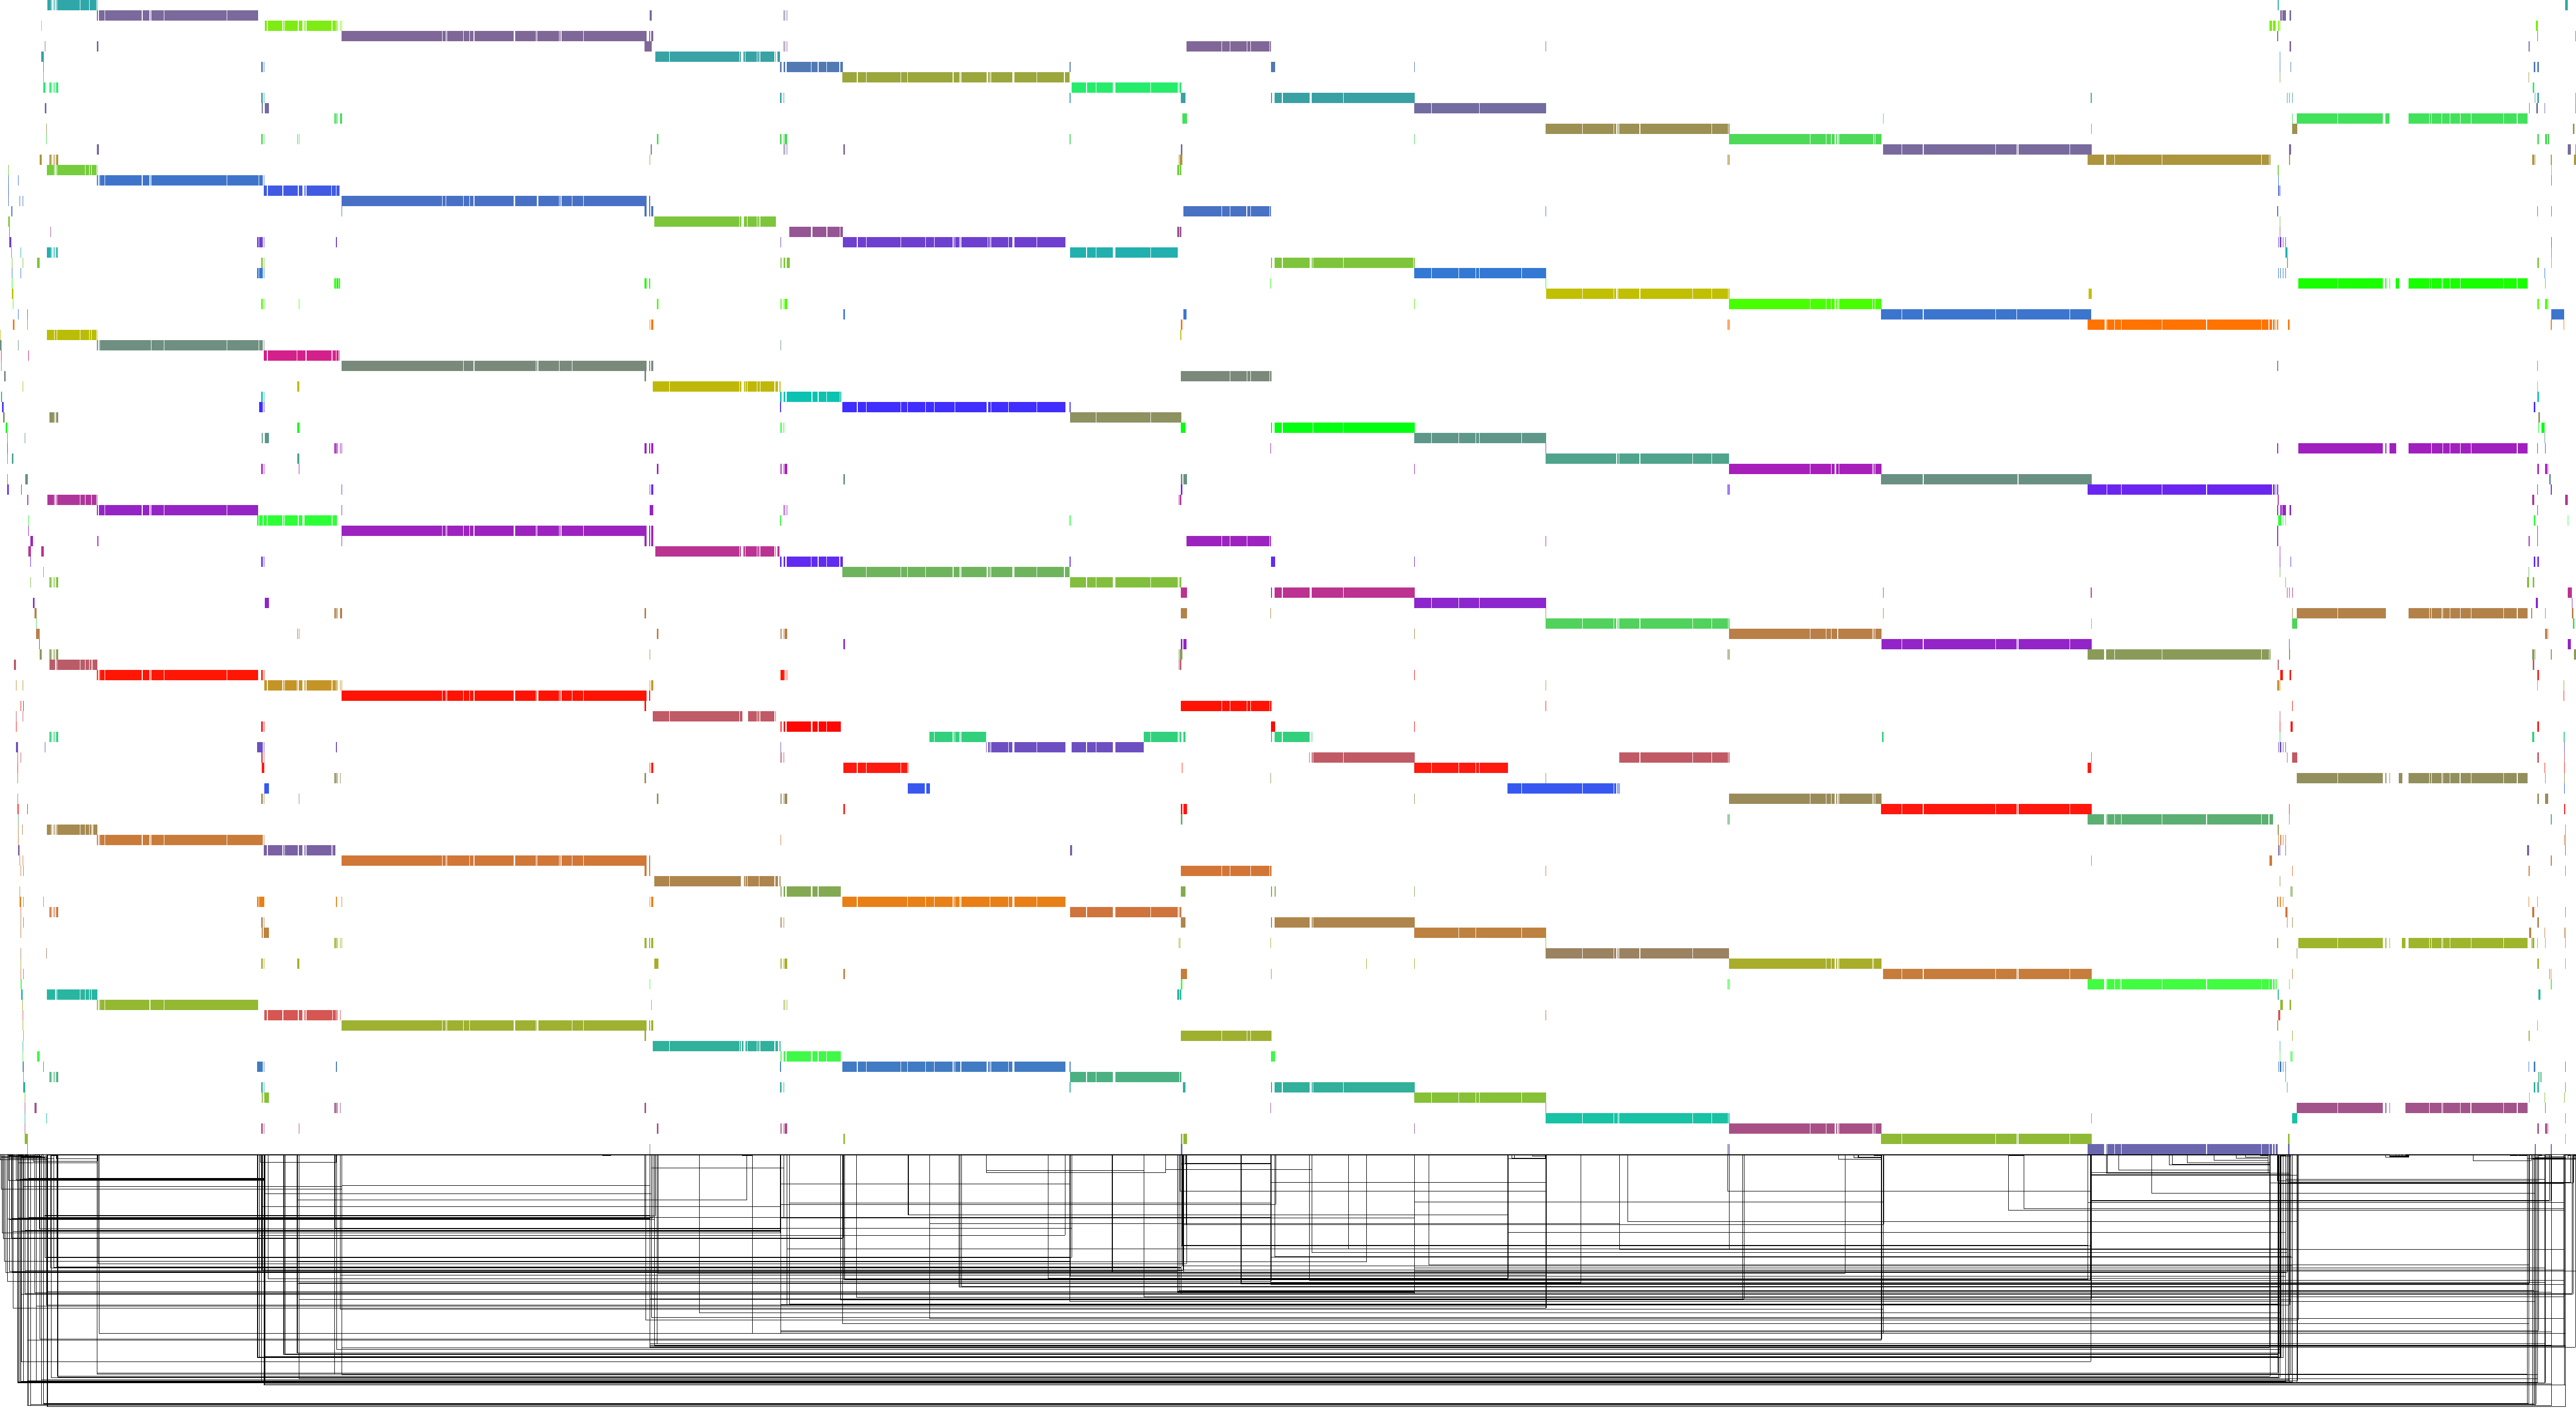
\includegraphics[scale=0.08,center]{seqwish-yeast-l10k-sort-dg.png}
  \end{figure}
\end{frame}

\end{document} 
